%&preformat-disser
\RequirePackage[l2tabu,orthodox]{nag} % Раскомментировав, можно в логе получать рекомендации относительно правильного использования пакетов и предупреждения об устаревших и нерекомендуемых пакетах
% Формат А4, 14pt (ГОСТ Р 7.0.11-2011, 5.3.6)
\documentclass[a4paper,14pt,oneside,openany]{memoir}

%% Режим черновика
\makeatletter
\@ifundefined{c@draft}{
  \newcounter{draft}
  \setcounter{draft}{1}  % 0 --- чистовик (максимальное соблюдение ГОСТ)
                         % 1 --- черновик (отклонения от ГОСТ, но быстрая сборка итоговых PDF)
}{}
\makeatother

%% Библиография

%% Внимание! При использовании bibtex8 необходимо удалить все
%% цитирования из  ../common/characteristic.tex
\newcounter{bibliosel}
\setcounter{bibliosel}{1}           % 0 --- встроенная реализация с загрузкой файла через движок bibtex8; 1 --- реализация пакетом biblatex через движок biber
               % общие настройки шаблона
\input{common/packages}  % Пакеты общие для диссертации и автореферата
\input{Dissertation/dispackages}         % Пакеты для диссертации
\input{Dissertation/userpackages}        % Пакеты для специфических пользовательских задач

%% Режим черновика
\makeatletter
\@ifundefined{c@draft}{
  \newcounter{draft}
  \setcounter{draft}{1}  % 0 --- чистовик (максимальное соблюдение ГОСТ)
                         % 1 --- черновик (отклонения от ГОСТ, но быстрая сборка итоговых PDF)
}{}
\makeatother

%% Библиография

%% Внимание! При использовании bibtex8 необходимо удалить все
%% цитирования из  ../common/characteristic.tex
\newcounter{bibliosel}
\setcounter{bibliosel}{1}           % 0 --- встроенная реализация с загрузкой файла через движок bibtex8; 1 --- реализация пакетом biblatex через движок biber
               % Упрощённые настройки шаблона

\input{Dissertation/preamblenames}       % Переопределение именований, чтобы можно было и в преамбуле использовать
% Новые переменные, которые могут использоваться во всём проекте
% ГОСТ 7.0.11-2011
% 9.2 Оформление текста автореферата диссертации
% 9.2.1 Общая характеристика работы включает в себя следующие основные структурные
% элементы:
% актуальность темы исследования;
\newcommand{\actualityTXT}{Актуальность темы.}
% степень ее разработанности;
\newcommand{\progressTXT}{Степень разработанности темы.}
% цели и задачи;
\newcommand{\aimTXT}{Целью}
\newcommand{\tasksTXT}{задачи}
% научную новизну;
\newcommand{\noveltyTXT}{Научная новизна:}
% теоретическую и практическую значимость работы;
%\newcommand{\influenceTXT}{Теоретическая и практическая значимость}
% или чаще используют просто
\newcommand{\influenceTXT}{Практическая значимость}
% методологию и методы исследования;
\newcommand{\methodsTXT}{Mетодология и методы исследования.}
% положения, выносимые на защиту;
\newcommand{\defpositionsTXT}{Основные положения, выносимые на~защиту:}
% степень достоверности и апробацию результатов.
\newcommand{\reliabilityTXT}{Достоверность}
\newcommand{\probationTXT}{Апробация работы.}

\newcommand{\contributionTXT}{Личный вклад.}
\newcommand{\publicationsTXT}{Публикации.}


\newcommand{\authorbibtitle}{Публикации автора по теме диссертации}
\newcommand{\vakbibtitle}{В изданиях из списка ВАК РФ}
\newcommand{\notvakbibtitle}{В прочих изданиях}
\newcommand{\confbibtitle}{В сборниках трудов конференций}
\newcommand{\fullbibtitle}{Список литературы} % (ГОСТ Р 7.0.11-2011, 4)

%Имена статистических моделей
\newcommand{\modelpphb}{P-Phb}
\newcommand{\modelpwhb}{P-Whb}
\newcommand{\modelwbr}{Wbr}
\newcommand{\modelCLS}{CLS}
\newcommand{\modelCRF}{CRF}
  % Новые переменные, которые могут использоваться во всём проекте

%%% Основные сведения %%%
\newcommand{\thesisAuthor}             % Диссертация, ФИО автора
{%
    \texorpdfstring{% \texorpdfstring takes two arguments and uses the first for (La)TeX and the second for pdf
        Алемасов Николай Александрович% так будет отображаться на титульном листе или в тексте, где будет использоваться переменная
    }{%
        Алемасов, Николай Александрович% эта запись для свойств pdf-файла. В таком виде, если pdf будет обработан программами для сбора библиографических сведений, будет правильно представлена фамилия.
    }%
}
\newcommand{\thesisAuthorShort}        % Диссертация, ФИО автора инициалами
{Н.А.~Алемасов}

\newcommand{\thesisUdk}                % Диссертация, УДК
{[577:616.8]/[004.94/004.42]}
\newcommand{\thesisTitle}              % Диссертация, название
{\texorpdfstring{\MakeUppercase{Компьютерный анализ связи между конформационными свойствами мутантных форм белка SOD1 и боковым амиотрофическим склерозом с использованием метода молекулярной динамики}}{Название диссертационной работы}}
\newcommand{\thesisSpecialtyNumber}    % Диссертация, специальность, номер
{\texorpdfstring{03.01.09}{XX.XX.XX}}
\newcommand{\thesisSpecialtyTitle}     % Диссертация, специальность, название
{\texorpdfstring{Математическая биология, биоинформатика}{Название специальности}}
\newcommand{\thesisDegree}             % Диссертация, ученая степень
{кандидата биологических наук}
\newcommand{\thesisDegreeShort}        % Диссертация, ученая степень, краткая запись
{канд. биол. наук}
\newcommand{\thesisCity}               % Диссертация, город написания диссертации
{Новосибирск}
\newcommand{\thesisYear}               % Диссертация, год написания диссертации
{2017}
\newcommand{\thesisOrganization}       % Диссертация, организация
{Федеральное государственное бюджетное научное учреждение <<Федеральный исследовательский центр Институт цитологии и генетики Сибирского отделения Российской академии наук>>}
\newcommand{\thesisOrganizationShort}  % Диссертация, краткое название организации для доклада
{ИЦиГ СО РАН}

\newcommand{\thesisInOrganization}     % Диссертация, организация в предложном падеже: Работа выполнена в ...
{Федеральном государственном бюджетном научном учреждении <<Федеральный исследовательский центр Институт цитологии и генетики Сибирского отделения Российской академии наук>>}

\newcommand{\supervisorFio}            % Научный руководитель, ФИО
{Иванисенко Владимир Александрович}
\newcommand{\supervisorRegalia}        % Научный руководитель, регалии
{к.б.н., доцент}
\newcommand{\supervisorFioShort}       % Научный руководитель, ФИО
{В.А.~Иванисенко}
\newcommand{\supervisorRegaliaShort}   % Научный руководитель, регалии
{к.б.н.,доц.}


\newcommand{\opponentOneFio}           % Оппонент 1, ФИО
{\todo{Фамилия Имя Отчество}}
\newcommand{\opponentOneRegalia}       % Оппонент 1, регалии
{\todo{доктор физико-математических наук, профессор}}
\newcommand{\opponentOneJobPlace}      % Оппонент 1, место работы
{\todo{Не очень длинное название для места работы}}
\newcommand{\opponentOneJobPost}       % Оппонент 1, должность
{\todo{старший научный сотрудник}}

\newcommand{\opponentTwoFio}           % Оппонент 2, ФИО
{\todo{Фамилия Имя Отчество}}
\newcommand{\opponentTwoRegalia}       % Оппонент 2, регалии
{\todo{кандидат физико-математических наук}}
\newcommand{\opponentTwoJobPlace}      % Оппонент 2, место работы
{\todo{Основное место работы c длинным длинным длинным длинным названием}}
\newcommand{\opponentTwoJobPost}       % Оппонент 2, должность
{\todo{старший научный сотрудник}}

\newcommand{\leadingOrganizationTitle} % Ведущая организация, дополнительные строки
{\todo{Федеральное государственное бюджетное образовательное учреждение высшего профессионального образования с~длинным длинным длинным длинным названием}}

\newcommand{\defenseDate}              % Защита, дата
{\todo{DD mmmmmmmm YYYY~г.~в~XX часов}}
\newcommand{\defenseCouncilNumber}     % Защита, номер диссертационного совета
{\todo{Д\,123.456.78}}
\newcommand{\defenseCouncilTitle}      % Защита, учреждение диссертационного совета
{\todo{Название учреждения}}
\newcommand{\defenseCouncilAddress}    % Защита, адрес учреждение диссертационного совета
{\todo{Адрес}}
\newcommand{\defenseCouncilPhone}      % Телефон для справок
{\todo{+7~(0000)~00-00-00}}

\newcommand{\defenseSecretaryFio}      % Секретарь диссертационного совета, ФИО
{\todo{Фамилия Имя Отчество}}
\newcommand{\defenseSecretaryRegalia}  % Секретарь диссертационного совета, регалии
{\todo{д-р~физ.-мат. наук}}            % Для сокращений есть ГОСТы, например: ГОСТ Р 7.0.12-2011 + http://base.garant.ru/179724/#block_30000

\newcommand{\synopsisLibrary}          % Автореферат, название библиотеки
{\todo{Название библиотеки}}
\newcommand{\synopsisDate}             % Автореферат, дата рассылки
{\todo{DD mmmmmmmm YYYY года}}

% To avoid conflict with beamer class use \providecommand
\providecommand{\keywords}%            % Ключевые слова для метаданных PDF диссертации и автореферата
{}      % Основные сведения
\input{common/styles}    % Стили общие для диссертации и автореферата
\input{Dissertation/disstyles}           % Стили для диссертации
\input{Dissertation/userstyles}          % Стили для специфических пользовательских задач
\input{biblio/bibliopreamble}% Настройки библиографии из внешнего файла (там же выбор: встроенная или на основе biblatex)

\input{Dissertation/inclusioncontrol}    % Управление компиляцией отдельных частей диссертации

\begin{document}

\input{common/renames}                   % Переопределение именований

% Структура диссертации (ГОСТ Р 7.0.11-2011, 4)
\include{Dissertation/title}           % Титульный лист
\include{Dissertation/contents}        % Оглавление
\include{Dissertation/introduction}    % Введение
\chapter{Литературный обзор} \label{chapt1}

\section{Боковой амиотрофический склероз} \label{sect_ALS}

Боковой амиотрофический склероз (БАС) -- заболевание, характеризующееся неотвратимой дегенерацией центральных и периферических моторных нейронов, приводящее к прогрессирующему параличу и возможной смерти от дыхательной недостаточности \cite{Alavi2013,Andersen2003,Drechsel2012,Haidet-Phillips2011}. Частота встречаемости заболевания составляет 1-2 случая на 100000 \cite{Alavi2013,Brotherton2012,Brown1997}.

БАС, как заболевание, был впервые описан в 1824 году Чарльзем Бэллом \cite{Rowland2001}. Большой вклад в описание патологии БАС внёс Жан Крювелье в 1852 году, а Француа Аран ещё в 1848 описал ряд случаев БАС, хотя не разделял заболевание по происхождению на нервное и мышечное \cite{Rowland2001, Marangi2015}. Сам термин <<боковой амиотрофический склероз>> был впервые упомянут в работе Жана Мартена Шарко в 1874 году \cite{Rowland2001}.

По разным данным от 1\% до 25\% случаев БАС имеют наследственную природу \cite{Abe1996,Alavi2013,Belzil2012,Eisen2008,Renton2011}. По данным секвенирования полного экзома человека, порядка тридцати генов вовлечены в заболевание БАС \cite{Cirulli2015}. Среди этих генов можно выделить следующие: \textit{SOD1}, \textit{TARDBP}, \textit{FUS}, \textit{OPTN} и \textit{VCP}. Взятые вместе, мутации в этих генах объясняют около 25\% наследственных случаев БАС \cite{Renton2011}. Кроме того, известен некодирующий регион C9orf72, в котором увеличенное количество шестинуклеотидных повторов GGGGCC также приводит к БАС \cite{Renton2011,DeJesus-Hernandez2011}.

\subsection{Некодирующий регион C9orf72} \label{subsect_C9orf72}

C9orf72 -- некодирующая область хромосомы 9, соответствующая открытой рамке считывания 72 \cite{DeJesus-Hernandez2011}. Было показано, что у здоровых людей максимальное количество повторов GGGGCC составило 23. У людей из выборки VSM-20 (по первым буквам организаций, выполнявших исследование: Vancouver, San Francisco и Mayo, семья 20), страдающих одним из заболеваний:  	лобно-височная деменция, БАС -- или обоими -- количество шестинуклеотидных повторов в C9orf72 варьировалось от 700 до 1600. На основе дополнительного анализа данных пациентов с БАС было выявлено $4.1$\% пациентов, страдающих спорадической формой заболевания и $23.5$\% пациентов -- наследственной формой, которые в то же время имели увеличенное количество повторов GGGGCC в C9orf72. 

Данный некодирующий участок хромосомы 9 изучался также другими авторами \cite{Renton2011}. При исследовании 405 финских пациентов и 497 здоровых людей обнаружено, что локус на хромосоме 9p21 объясняет до четверти всех случаев БАС и до половины всех случаев его наследственной формы \cite{Laaksovirta2010}. В последующем исследовании также был выделен участок C9orf72, количество шестинуклеотидных повторов GGGGCC в котором отделяло здоровых людей от больных БАС \cite{Renton2011}. На основе анализа данных от нескольких семей с БАС, обнаружено, что у здоровых людей повторов было меньше 20, а у больных -- больше 30. Анализ 402 финских пациентов с БАС и 478 здоровых людей выявил, что количество шестинуклеотидных повторов увеличено у $28.1$\% пациентов и $0.4$\% здоровых людей. Всего пациентов с наследственной формой БАС, у которых увеличено количество повторов  GGGGCC, оказалось $46.4$\%, а среди пациентов со спорадической формой заболевания было $21$\% с повышенным числом повторов. В среднем количество повторов у пациентов было 53, у здоровых людей -- 2. Таким образом, C9orf72 отвечает за наибольшее количество случаев заболевания БАС. 

\subsection{Ген \textit{SOD1}} \label{subsect_SOD1}

Другой наследственной причиной развития БАС являются мутации в гене \textit{SOD1}, кодирующем фермент супероксиддисмутазу-1 \cite{Bosco2010,Ivanova2014}. На данный момент известно свыше 170 мутаций этого гена, вызывающих различные формы БАС (http://alsod.iop.kcl.ac.uk/). 

Белок супероксиддисмутаза-1 (SOD1) -- гомодимер. Он катализирует реакцию превращения анионов супероксида на молекулярный кислород и пероксид водорода. Каждая из двух субъединиц белка состоит из 153 аминокислотных остатков и содержит в себе два иона: медь и цинк. Каждая субъединица имеет в своей вторичной структуре $\beta$-бочонок, составленный из 8 $\beta$-тяжей, и две функционально важных петли: электростатическую и цинк-связывающую. Также в субъединицах присутствует по одной дисульфидной связи.

\todo{\cite{Das2013}}

\subsection{Ген \textit{TARDBP}} \label{subsect_TARDBP}

Мутации в белке TDP-43, кодируемом геном \textit{TARDBP} также приводят в $1$\% случаев к заболеванию БАС, как наследственной, так и спорадической формы \cite{Corrado2009}. Заметные включения, содержащие убиквитин, как считается, являются признаком этого заболевания \cite{Kabashi2008,VanDeerlin2008}. В то же время среди белков, составляющих агрегат главный компонент -- TDP-43 \cite{Sreedharan2008,Kabashi2008,Kuhnlein2008}. TDP-43 -- РНК-связывающий и ДНК-связывающий белок, имеющий множество функций в клетке. Изначально TDP-43 был классифицирован, как репрессор транскрипции, который связывается с TAR-элементом ВИЧ. Из-за своего молекулярного веса он был назван TDP-43 \cite{VanDeerlin2008}. Белок TDP-43 участвует в регуляции экспрессии генов и сплайсинге, присутствует в комплексе, который производит сплайсинг гена \textit{CFTR} и, вероятно, также участвует в биогенезе микро-РНК, апоптозе и клеточном делении \cite{Sreedharan2008,VanDeerlin2008}. Известно, что накопление гиперфосфорилированных фрагментов TDP-43 в перикарии нейронов у пациентов с БАС связано со значительной потерей TDP-43 в ядре \cite{Sreedharan2008}. За исключением одной, все известные мутации TDP-43 сосредоточены в C-терминальной части белка -- глицин-богатом районе, который, вероятно, участвует в связывании с другими белками, включая разнообразные рибонуклеопротеины \cite{Corrado2009}. Кроме того, подтверждено наличие в образцах мозга пациентов с БАС меньшей фосфорилированной части (25 кДа) C-концевого фрагмента TDP-43, а также крупных убиквитинированных агрегатов, включающих данный белок \cite{Corrado2009}. Обнаружено, что TDP-43 связывается с высокой аффинностью с убиквилином-2 (UBQLN2) -- подобным убиквитину белком семейства UBQLN \cite{Cassel2013}. Мутации в UBQLN2 известны в качестве генетического маркера доминантного X-сцепленного варианта возникновения БАС. Вместе с тем UBQLN2 усиливает выведение, как TDP-43, так и C-концевых фрагментов, то есть может влиять на цитотоксичность \cite{Cassel2013}.

%\newpage
%============================================================================================================================

\section{Агрегация белков} \label{sect_aggregation}

Эукариотические клетки -- сложные структуры, способные разграничивать происходящие внутри биохимические реакции в пространстве и времени. Ключевым механизмом такого разграничения является разделение внутриклеточного пространства на функциональные области. Один из хорошо известных примеров таких разделённых областей -- клеточные органеллы, отделённые от внешнего пространства внутриклеточными мембранами, действующими, как физический барьер. Последние исследования открыли также немембранный способ разграничения реакций -- так называемое <<расслоение жидкостей>> (liquid demixing) -- разделение различных растворов, находящихся в жидкой фазе \cite{Aguzzi2016}. Этот способ, по-видимому, используется клеткой для динамической перестройки внутриклеточного пространства. Например, когда требуется временно провести некоторую реакцию в ограниченной от других реакций области. Так, для функционально неупорядоченных белков (от англ. Intrinsically disordered proteins) вероятность фазового разделения должна быть довольно высокой, поскольку данный тип белков из-за своей структурной гибкости способен создавать множественные взаимодействия с другими белками.

Известны примеры функционального расслоения жидкостей в эукариотических клетках: ядрышко, P-гранулы (околоядерные РНК-гранулы), стрессовые РНК-гранулы, тельца Кахаля, <<ядерные пятна>> (paraspeckles), P-тела (processing (P) bodies) \cite{Aguzzi2016}. Фактически, механизм разделения жидких фаз является универсальным, в частности, для образования частиц рибонуклеопротеинов. Другими примерами немембранных многобелковых комплексов являются центросомы, сигнальные молекулы (мембранные рецепторы) и ядерные поры.

В рамках данной парадигмы разделения фаз выделяются три различных состояния, в которых могут находиться молекулы в клетке: рассеянное (газообразное), жидкое, твёрдое \cite{Aguzzi2016}. Применительно к белкам, газообразное состояние соответствует раствору, в котором белки находятся отдельно друг от друга; жидкое состояние -- растворимым белковым комплексам, отделённым <<расслоением жидкости>>; твёрдое -- нерастворимым белковым агрегатам.

Как уже упоминалось, белки, находящиеся, в <<жидкой фазе>> имеют большое количество функциональных взаимодействий засчёт конформационной подвижности присутствующих в них неупорядоченных областей и областей с низкой сложностью аминокислотного состава (low complexity regions). При этом, известно, что белки с более протяжёнными неупорядоченными участками имеют меньшее время существования в клетке \cite{VanderLee2014}. Для белков, не подверженных и подверженных агрегации наблюдается аналогичная закономерность: чем более белок подвержен агрегации, тем более быстрый <<круговорот>> в клетке он имеет и тем более низкая его концентрация поддерживается \cite{Gsponer2012}.

\todo{С этой точки зрения агрегация ряда белков, которая приводит к различным заболеваниям человека, должна возникать из-за нарушения механизма деградации этих белков или механизма поддержания их низкой концентрации.}

\todo{С этой точки зрения белки с мутацией, которая могла бы препятствовать нормальной деградации должны существовать дольше и, наряду с приобретённым в связи с мутацией новым, нежелательным взаимодействием или функцией, тем самым, могут образовывать более стабильные белковые агрегаты.}

\todo{Накопление в нервных клетках убиквитинированных включений является признаком того, что протеасома более не справляется с переработкой повреждённых белков \cite{Sreedharan2008}.}

\todo{\cite{MadanBabu2016}}

\section{Белок SOD1 и его мутации} \label{sect_SOD1}

На молекулярном уровне мутации приводят к различным изменениям в структуре белка SOD1. Одним из следствий мутации белков SOD1 является образование внутриклеточных агрегатов \cite{Bruijn1998,Deng2006}. Предложено большое количество объяснений агрегации SOD1 \cite{Ross2004}. В соответствии с одной из этих гипотез, причиной агрегации мутантных SOD1 становится снижение их стабильности при удалении ионов металлов \cite{Bourassa2014}. Другой вероятной причиной являются посттрансляционные модификации SOD1, выделенных из тканей человека, которые снижают стабильность димера \cite{Dokholyan2015}.

\section{Конформационные свойства белков} \label{sect_proteins_features}

\section{Компьютерные методы анализа белков} \label{sect_computational_methods}

\subsection{Метод молекулярной динамики} \label{sect_methods_MD}

Важнейшим средством теоретического исследования структуры, динамики и термодинамических свойств комплексов биомакромолекул является метод молекулярной динамики (МД), который является методом компьютерного моделирования, позволяющим в течение заданного периода времени проследить эволюцию системы взаимодействующих атомов с помощью численного интегрирования уравнений движения \cite{Alder1957,Gibson1960}. Метод МД широко используется для решения задач исследования термостабильности белков, конформационных переходов, транспорта молекул, белкового фолдинга и прочих. К сожалению, разброс масштабов различных физических явлений огромен, от $10^{-8}$ сек (времена движения доменов) до 1-10 сек (время самоорганизации белков и нуклеиновых кислот), и находится вне возможностей современной МД. По этой причине исследования конформационных переходов макромолекул в настоящее время сделаны только для систем малых белков и пептидов \cite{Zhou2002,Nymeyer2003}, а для больших систем, размером более 1 млн. атомов, траектории исследовались в ограниченном временном интервале не превышающем 50 нс \cite{Freddolino2006}. 

Метод молекулярной динамики состоит в численном интегрировании уравнений движения Ньютона для системы взаимодействующих частиц (атомов), находящихся в некоторых начальных условиях (заданы начальные координаты и скорости каждого атома):

\[
F_i = -\frac{\partial U(r_1,\ldots,r_N)}{\partial r_i}
\]

где i = 1 \ldots N,--координаты атома i; N--количество атомов.

Движение атомов описывается уравнениями:

\begin{equation}
\label{eq:newton_motion}
\frac{d^2r_i}{dt^2}=\frac{F_i}{m_i}
\end{equation}

где $m_i$--масса атома i.

Типичное МД-исследование предполагает расчёт траектории развития системы во времени и её изучение на предмет интересующих свойств. При этом точность расчётов зависит от выбранной функции потенциальной энергии U, форма которой вместе с необходимыми для её использования параметрами составляют силовое поле. 

\subsubsection{Силовое поле} \label{sect_methods_forcefield}

В соответствии с квантовой теорией, для небольших молекул энергия системы может быть определена методами квантовой химии. Но при числе атомов более десяти задача становится трудно вычислимой \cite{Shaitan2006}. Поэтому в МД применяются такие потенциалы, которые зависят только от положения атомов, что позволяет исследовать системы с десятками-сотнями тысяч и даже миллионами атомов.

В существующих силовых полях МД функция потенциальной энергии разбивается на сумму вкладов от различных типов взаимодействий: $U = U_b+U_\theta+U_\Phi+U_{el}+U_{LJ}$. Среди них взаимодействия:

\begin{enumerate}

\item Ближние

	\begin{enumerate}

	\item Связующие

		\begin{enumerate}

		\item растяжение связей:
		
		\[
		U_{b} = \frac{1}{2} \sum_b{K_{b}(r-b_{0})^{2}}
		\]
		
		где $b_0$--равновесная длина связи; $K_b$--силовая константа.
		
		\item изменение валентных углов:
		
		\[
		U_{\theta} = \frac{1}{2} \sum_\theta{K_{\theta}(\theta-\theta_{0})^{2}}
		\]
		
		где $\theta_0$--равновесное  значение угла; $K_{\theta}$- силовая константа.

		\item изменение двугранных углов:

		\[
		U_{\Phi} = \sum_{\Phi}{K_{\Phi}[cos(n\Phi-\delta)+1]}
		\]
		
		где $n$--кратность торсионного барьера; $\delta$--сдвиг фазы; $K_{\Phi}$--константа, определяющая высоту потенциальных барьеров двугранных углов.

		\end{enumerate}

	\item Несвязующие 
	
	Возникают между парами атомов, принадлежащими различным молекулам. Либо принадлежащие той же самой молекуле, но разделённые, по крайней мере, тремя связями.

		\begin{enumerate}
	
		\item электростатические:
		
		\[
		U_{el} = \sum \frac{q_{i} q_{j}}{\epsilon r_{ij}}
		\]

		где $q_i$, $q_j$--парциальные заряды на атомах; $\epsilon$--диэлектрическая проницаемость среды.
		
		\item  ван-дер-ваальсовы:
		
		\[
		U_{LJ} = \sum{\left [ \frac{A}{r_{ij}^{12}}-\frac{B}{r_{ij}^{6}} \right ]}
		\]
		
		где $A$, $B$ зависят от типов атомов $i$ и $j$; $r_{ij}$— расстояние между этими атомами.

		\end{enumerate}

	\end{enumerate}

\item  Дальние электростатические

В этом случае кулоновский потенциал разбивается на две части--ближнюю и дальнюю:

\[
U_{el} = \sum { \frac{1 - erf(\beta r_{ij})}{\epsilon r_{ij}}} q_i q_j + \sum {\frac{erf(\beta r_{ij})}{\epsilon r_{ij}}} q_i q_j
\]

Здесь дробь в первой сумме ведёт себя как $1/r$ при $r \to 0$, убывает экспоненциально при $r \to \infty $ и отвечает за ближнюю часть взаимодействий, вторая дробь стремится к $1/r$ при $r \to \infty $ и отвечает за дальнюю часть. $\beta$--параметр, определяющий относительный вклад между прямой суммой и суммой в обратном пространстве (см. раздел \ref{subsubsect_methods_MD_concepts}), $erf(x) = \frac {2}{\sqrt{\pi}} \int_0^x{e^{-t^2} dt}$--функция ошибки.

\end{enumerate}

Параметры силовых полей для потенциалов взаимодействий определяются из различных экспериментальных данных (спектральные, калориметрические, кристаллографические) и квантово-химических расчётов. Наиболее часто используются такие поля, как: AMBER \cite{Cornell1995,Kollman1996,Wang2000,Hornak2006,LindorffLarsen2010,Duan2003,Garcia2002}, CHARMM \cite{Mackerell2004,Mackerell1998,Feller2000,Foloppe2004}, GROMOS \cite{Gunsteren1996}, OPLS \cite{Jorgensen1996}, CVFF (CFF, PCFF) \cite{Hagler1974}.

\subsubsection{Основные концепции МД} \label{subsubsect_methods_MD_concepts}

В своей основе МД содержит простой принцип, но дополнительные приёмы позволяют превратить этот принцип в практически полезный инструмент.

Первый шаг алгоритма моделирования предполагает расчёт сил, действующих на каждый из атомов, используя силовое поле. С изменением положения атома меняются и силы, поэтому исходные уравнения движения не могут быть разрешены аналитически--их интегрируют численно.

Интегрирование разделяется на небольшие шаги, отличающиеся между собой по времени на $\Delta t$. После того как силы рассчитаны для текущей (на время $t$) конфигурации атомов, следующим шагом является генерация новой конфигурации на момент времени $t+\Delta t$, используя уравнение \eqref{eq:newton_motion}. Координаты атомов приблизительно вычисляются с помощью ряда Тейлора:

\[
r(t+\Delta t) = r(t) + \Delta t {\frac{d}{dt}} r(t) + { \frac{(\Delta t)^2}{2!} } {\frac{d^2}{dt^2}} r(t) + \ldots
\]

В настоящий момент при моделировании МД наиболее всего распространён метод интегрирования Верле \cite{Verlet1967}. Для координат и скоростей он записывается:

\[
r_i(t + \Delta t) \approx -r_i(t - \Delta t) + 2r_i(t) + \Delta t^2 {\frac{F_i}{m_i}}
\]

\[
v_i(t) \approx {\frac{1}{2 \Delta t}} [r_i(t + \Delta t) - r_i(t - \Delta t)]
\]

Одной из модификаций этого алгоритма является leap-frog схема \cite{Hockney1974}:

\[
r_i(t + \Delta t) \approx r_i(t) + \Delta t v_i(t + \frac{\Delta t}{2})
\]

\[
v_i(t + \frac{\Delta t}{2}) \approx v_i(t - \frac{\Delta t}{2}) + \Delta t \frac{F_i}{m_i}
\]

При моделировании макромолекул шаг интегрирования выбирается равным десятой доли самого короткого периода движения. Самые быстрые движения--растяжения связей, особенно соединённых с водородом. C-H колебания имеют период около 10 фс (1 фс = $10^{-15}$ сек), что даёт шаг интегрирования порядка 1 фс.

Начальные условия для координат и скоростей задаются по-разному. Координаты атомов выбираются в соответствии с геометрией и структурой моделируемой молекулярной системы. Например, координаты атомов белков, могут быть получены с помощью рентгеноструктурного анализа или метода ЯМР. Начальные скорости же задаются с помощью генератора случайных чисел, имеют максвелловское распределение и соответствуют выбранной температуре.

Обычно размер модели и самой моделируемой системы не совпадают. Сложно представить, например, моделирование целой мембраны, которое бы могло быть проведено в достаточно короткий срок. Для решения этой проблемы используются периодические граничные условия. Молекулярная система помещается в <<ящик>>, окружённый со всех сторон своими виртуальными образами. Таким образом, атом, который пересёк границу ящика появляется с противоположной его стороны.

Другой проблемой является расчёт парных, несвязующих взаимодействий. В принципе, парные взаимодействия рассчитываются для каждой пары атомов в системе, но это приводит к числу пар, равному квадрату числа атомов. С другой стороны, закон распространения несвязующих взаимодействий таков, что они быстро убывают с ростом расстояния. Поэтому часть пар не вносят существенного вклада в энергию. Такие пары можно исключить из расчёта, введя так называемый радиус отсечения. Пары, атомы которых расположены дальше друг от друга, чем установленный радиус отсечение в расчёте не участвуют. Значения устанавливаемых радиусов обрезания обычно лежат в промежутке от 8 до 12~\AA.

Применение радиуса отсечения при расчёте дальних электростатических взаимодействий может быть не достаточно точным. Полная электростатическая энергия представляет собой сумму для N атомов в решётке (nx, ny, nz) = n:

\[
U_{el} = \frac{f}{2} \sum_{n_x}\sum_{n_y} \sum_{n_z} \sum_{i}^{N}\sum_{j}^{N} {\frac{q_i q_j}{r_{ij,\bold n }}}
\]

где $r_{ij,\bold n}$--расстояние между зарядами (но не между ближайшими образами). 

Однако эта сумма сходится медленно. В этом случае учёт взаимодействий типа заряд-заряд должен быть с использованием таких методов как, например, метод суммирования Эвальда \cite{Ewald1921}, метод Particle-Mesh Ewald (PME) \cite{Darden1993,Essmann1995}, метод Particle-Particle Particle-Mesh (PPPM или P${}^3$M) \cite{Hockney1981,Luty1995} или метод Isotropic Periodic Sum (IPS) \cite{Wu2005}. Эти алгоритмы производят полное суммирование сил между бесконечным количеством образов атомов системы (из-за периодичных граничных условий) в обратном пространстве Фурье, что улучшает сходимость. Метод суммирования Эвальда имеет сложность порядка $N^{3/2}$, PME и PPPM имеют трудоёмкость порядка $N\log N$. Ключевое отличие метода IPS от методов, использующих решётку (например, PME) в форме и распределении образов частиц. В PME образы частиц идентичны образам частиц, получаемым в периодических граничных условиях и дискретно расположены в узлах решётки. В IPS же образы частиц не совпадают с реальными, что означает, что они не существуют реально. И, в то же время, «воображаемые» образы распределены изотропным и периодическим образом вокруг частицы. Для полностью гомогенных систем IPS-образы распределены одинаково во всех трёх измерениях. Для большинства типов потенциалов существует аналитическое решение в трёхмерном IPS.

МД даёт микроскопическое описание развития системы. Чтобы перейти от микроскопического описания к макроскопическому приходится использовать статистическую механику. Среди макроскопических параметров--температура (T), давление (P), объём (V), число частиц (N), внутренняя энергия (E), химический потенциал ($\mu$).

Микроскопическое состояние системы описывается положением каждого атома $r$ и импульсом $p$ \cite{Gibbs1946}. Таким образом, чтобы представить систему в обобщённом пространстве потребуется указать 6 параметров (для трёх измерений; 3 компоненты координаты, 3--импульса). Подобное обобщённое пространство называется фазовым пространством. Мгновенное состояние системы можно представить в виде точки в фазовом пространстве. Соответственно, развитие системы--в виде множества точек--траектории.

Различают несколько типов совокупностей состояний системы, удовлетворяющих определённым условиям (ансамблей), в которых может проходить моделирование МД:

\begin{enumerate}
\item Микроканонический (NVE). Постоянными являются: число атомов (N), объём (V), и энергия (E).
\item Канонический (NVT). Постоянные: число атомов (N), объём (V) и температура (T).
\item Изобарно-изотермический (NPT). Постоянные: число атомов (N), давление (P) и температура (T).
\item Большой канонический ($\mu$VT). Постоянные: химический потенциал ($\mu$), объём (V) и температура (T).
\end{enumerate}

Термодинамические свойства могут рассчитываться МД путём усреднения по времени. В эксперименте же усреднение происходит по всему набору состояний, которые принимает система, то есть--усреднение по ансамблю. Это несоответствие разрешается с помощью эргодической гипотезы \cite{Ulenbek1965}, которая говорит, что среднее по времени равно среднему по ансамблю. Ключевой момент этого равенства--в идее того, что за время движения системы в фазовом пространстве она успевает посетить все точки этого пространства, то есть принять все возможные состояния. Фактически же для моделирования этого достичь невозможно, поскольку для систем, которые обычно моделируются фазовое пространство огромно. Но, используя различные методы становится возможным генерировать достаточно представительные наборы состояний, которые дают довольно точные результаты.

Мгновенная температура системы определяется через среднюю кинетическую энергию входящих в систему частиц:

\[
T(t) = {\frac{1}{3 N k_B}} \sum_{i=1}^N {m_i v_i^2(t)}
\]

где $N$--число атомов; $k_B$--константа Больцмана; $m_i$--масса атома $i$; $v_i$--его скорость. 

Эффективная температура системы определяется как среднее по времени: $T = \left \langle T \right \rangle$ в течение достаточно длинного временного интервала.

При моделировании обычно возникает потребность установить определённую температуру системы. Это делается с помощью установки скоростей атомов с гауссовым распределением. Однако, в процессе моделирования из-за ошибок округления температура может изменяться. Поэтому её корректируют, используя схему Берендсена \cite{Berendsen1984} или более расширенную--Нозе-Гувера \cite{Nose1984,Hoover1985}, а также модифицированную схему Берендсена \cite{Bussi2007}.

Алгоритм Берендсена предполагает соединение молекулярной системы с термостатом, который поставляет в систему или выводит из неё тепло, если потребуется. Температура системы корректируется через:

\[
{\frac{dT(t)}{dt}} = {\frac{1}{\tau}} (T_0 - T(t))
\]

где $\tau$--временная константа, определяющая величину коррекции; $T_0$--температура термостата.
В соответствии с этим соотношением, скорости масштабируются с параметром $\lambda$:

\[
\lambda = \left [1 + {\frac{\Delta t}{\tau_T}} \left ( {\frac{T_0}{T(t)}} - 1 \right ) \right ]^{\frac{1}{2}}
\]

Недостатком этого метода является неравномерное распределение энергии по степеням свободы. Разные части системы принимают различные температуры, что приводит к проблеме \cite{Harvey1998}. 

Использование более сложного термостата Нозе-Гувера предполагает его введение в саму систему, предоставляя дополнительную степень свободы. Однако, это также не приводит к физическому распределению энергии по степеням свободы \cite{Golo2004}.

Модифицированная схема Берендсена (или V-rescale термостат) добавляет случайный множитель к генерируемым скоростям, что позволяет получать корректное распределение для кинетической энергии.

Расчёт давления в МД соответствует следующему определению. Для <<ящика>> со стороной $L$ с внедрённой в него плоской поверхностью площадью $A = L^2$, ориентированной перпендикулярно оси $x$, имеем давление на эту поверхность:

\[
P_x=\frac{F_x}{A}
\]

Из второго закона Ньютона это соотношение переписывается в виде:

\[
P_x = {\frac{1}{A}} {\frac{d(m v_x)}{dt}}
\]

Таким образом, давление представляет собой <<количество>> импульса, проходящего через заданную площадь за единицу времени. Этот <<поток импульса>> состоит из двух частей: импульса атомов при пересечении площадки за время $dt-P_m$ и импульса от действия сил на атомы, лежащие по разные стороны от площадки $P_f$. 

\[
P_x=P_{mx}+P_{fx}
\]

В соответствии с молекулярно-кинетической теорией в случае идеального газа давление $P_m$ определяется, как:

\[
\langle P_m \rangle = \frac{2 N}{3 V} \langle E_k \rangle
\]

где $V$--объём; $N$--число атомов; $E_k$--кинетическая энергия в расчёте на один атом; угловые скобки означают усреднение по времени.

Давление, обусловленное действием сил между противоположными относительно воображаемой площадки, Pfx, предполагая, что эти силы попарно суммируются: 

\[
P_{fx} = \frac{1}{A} \sum_i \sum_j {F_{ij} \cdot x}
\]

где $x$--единичный вектор в положительном направлении x; $i$ пробегает по всем атомам одной стороны площадки, $j$--по атомам другой её стороны.

Усредняя по всем возможным положениям воображаемой площадки вдоль оси x, а также учитывая аналогичные выражения для площадок, расположенных перпендикулярно осям y и z, имеем полный вклад:

\[
\langle P_f \rangle = \frac{1}{3 V} \left \langle \sum_i \sum_j {F_{ij} \cdot r_{ij}} \right \rangle
\]

Сложив выражения для $P_m$ и $P_f$ получим выражение для давления в зависимости от мгновенных скоростей, координат и сил в системе:

\[
P = \frac{2 N}{3 V} E_k + \frac{1}{3 V} \sum_i \sum_j {F_{ij} \cdot r_{ij}}
\]

Большинство реальных экспериментов проводятся при постоянных температуре и давлении, что делает естественным стремление проводить моделирование в NPT-ансамбле, чтобы иметь возможность напрямую сравнивать результаты моделирования с экспериментальными данными. Методы установки давления аналогичны методам для установки температуры--система может быть соединена с баростатом, который будет поддерживать постоянное давление, регулируя объём ящика моделирования множителем $\mu$:

\[
\mu = 1 - \kappa {\frac{\Delta t}{\tau_p}} (P - P_0)
\]

где $\kappa$--коэффициент изотермической сжимаемости; $\tau_p$--константа релаксации; $P_0$--давление баростата; $P$--мгновенное давление на момент времени $t$; $\Delta t$--временной шаг.

Масштабирование объёма со множителем $\mu$ эквивалентно масштабированию координат со множителем. Причём множители могут быть неодинаковыми для масштабирования по различным осям. Более сложный метод поддержания давления реализуется с помощью алгоритма Паринелло-Рамана \cite{Parrinello1981}, который подобен термостату Нозе-Гувера.

В процессе моделирования система включает движения различных частот, наивысшие из которых принадлежат колебаниям длин связей. Именно наивысшие частоты определяют минимальный временной шаг: чем выше частота, тем меньше шаг--что влияет на конечное время моделирования. Кроме того, наибольшее влияние на конформацию молекулы оказывают низкочастотные движения. Поэтому идея <<удаления>> высокочастотных перемещений атомов вполне закономерна. Например, можно сделать связи жёсткими, ограничивая длины связей без ущерба точности вычислений. Существует ряд методов, позволяющих ввести так называемые ограничения в МД, один из которых--метод SHAKE \cite{Ryckaert1977}.

В методе SHAKE на атомные координаты накладываются голономные (зависящие только от координат) ограничения:

\[
\sigma(r_1, r_2, \ldots r_N) = 0
\]

где $N$--число атомов с количеством степеней свободы $3N$.

Если есть $k$ голономных ограничения, то общее число степеней свободы составит $3N-k$. В соответствии с этими ограничениями на атомы действуют два типа сил: молекулярные (которые присутствовали в системе до введения ограничений), а также силы, обусловленные ограничениями. Последний тип сил выглядит так:

\[
G_i = - \sum_{k=1}^K {\lambda_k \frac{\partial \sigma_k}{\partial r_i}}
\]

где $K$--количество ограничений; $\lambda_k$--множители Лагранжа.

Полная сила для атома $i$ записывается в этом случае следующим образом:

\[
F_i^{'} = F_i + G_i = - {\frac{\partial}{\partial r_i}} \left ( U(r) + \sum_{k=1}^K {\lambda_k \sigma_k} \right )
\]

Разрешая набор множителей Лагранжа, алгоритм может столкнуться с ситуацией, когда одно ограничение не позволяет удовлетворить другое. Поэтому требуется совершение нескольких итераций для того, чтобы удовлетворить все ограничения (с некоторым допуском). Похожий на SHAKE алгоритм--SETTLE \cite{Miyamoto1992}--используется для превращения молекул воды в жёсткие структуры. Помимо перечисленных, например, в пакете программ GROMACS используется метод LINCS \cite{Hess1997}, который <<сбрасывает>> длины связей на их начальные значения.

\subsection{Метод эластичных сетей} \label{subsect_methods_EN}

Метод МД для полноатомных моделей белка ограничен в своей применимости для получения протяжённых по времени моделирования траекторий. Это, в первую очередь, вызвано трудоёмкостью вычислений. Например, для того, чтобы получить траекторию МД изучаемой структуры белка SOD1 протяжённостью 50 нс, было затрачено 90 часов работы одного вычислительного узла высокопроизводительного кластера, оснащённого тремя ускорителями Tesla. Отслеживание конформационных переходов в структуре белка требуют значително большего времени моделирования--от микросекунд до миллисекунд \cite{Ding2008}. Методом МД моделирование полноатомных представлений белка потребовали бы до десятков лет расчётов. 

По этой причине для решения таких задач часто используются упрощённые модели белков, такие как, например, крупнозернистые (coarse grained) модели \cite{Rudd1998} или представления структуры белка в виде эластичной сети (elastic networks) \cite{Tirion1996}. Суть крупнозернистых приближений структуры белка состоит в том, чтобы заменить целую группу атомов одной частицей. Это позволяет снизить количество степеней свободы всей молекулярной системы и, таким образом, перейти на более крупный масштаб динамики белка. В эластичных моделях количество атомов остаётся неизменным, но потенциалы взаимодействия между ними заменяются на более простые, например, однопараметрический гармонический потенциал (аналог пружины).

Мода колебаний

Коллективность

Какие методы ещё есть? 
Для чего использовались? 
Что обнаружено? 
Какие результаты?

           % Глава 1
\chapter{Методы, используемые для определения динамических свойств структуры мутантов белка SOD1} \label{chapt2}

\section{Моделирование методом молекулярной динамики} \label{sect_MD}

\subsection{Протокол моделирования} \label{subsect_MD_protocol}

В работе для моделирования в рамках метода молекулярной динамики был применён программный комплекс AMBER 12 \cite{Salomon-Ferrer2013}. В качестве аппаратной платформы выступал гибридный высокопроизводительный кластер ЦКП <<Биоинформатика>> (http://bioinformatics.bionet.nsc.ru/), который содержит ускорители NVIDIA Tesla M2090. Для анализа структуры использовалась программа UCSF Chimera \cite{Pettersen2004}. Статистическая обработка велась с помощью языка Python 2.7 и пакетов scipy, numpy, sklearn \cite{Pedregosa2011}, scikits.bootstrap. Графика подготовлена с помощью пакета matplotlib, DOG 2.0 \cite{Ren2009} и UCSF Chimera.

При моделировании МД применён следующий набор параметров: шаг интегрирования--2 фс; радиус отсечения взаимодействий--10~\AA; температура--300 К; время моделирования--50 нс. В качестве модели воды использовалась TIP3P. Кубическая ячейка имела сторону 12~\AA и состояла из более чем 20000 молекул воды, растворённого в ней белка (PDB ID: 2V0A) из 4376 атомов. В зависимости от заряда мутантного белка в <<раствор>> добавлялось порядка 36 и 30 соответственно ионов Na+ и Cl-, что соответствовало концентрации 0.137 моль.  Для обеспечения достоверности результатов моделирования каждая траектория МД повторялась 5 раз. В итоге для 40 форм белка было получено 200 траекторий, общей протяжённостью  10~мкс.

Параметры сайта связывания атома цинка получены с помощью расчётов в рамках теории функционала плотности (DFT). Был применён обменный функционал M06 с базисным набором 6–31+G* \cite{Zhao2007} из пакета Gaussian 09 \cite{Frisch2009} с эталонной экспериментальной структурой (PDB ID: 2V0A). Далее, параметры были адаптированы для силового поля с помощью модуля MTK++/MCPB \cite{Peters2010} из пакета программ AmberTools14.

Белок для нормального функционирования в клетке требует включения в свой состав ионов меди и цинка. Известно, что количество атомов меди \~0.2/димер, а цинка \~1.5/димер \cite{Ayers2014}, что говорит о том, что моделирование может осуществляться без учёта иона меди. 

Параметры \modelpphb{}, \modelpwhb{} и \modelwbr{} были получены путём анализа траектории МД утилитой cpptraj из комплекса программ AMBER. Утилита cpptraj обнаруживает водородные связи внутри белка и между атомами белком и окружающими его молекулами воды, а также водные мостики, возникающие между аминокислотными остатками белка и возвращает время существования каждой обнаруженной связи, нормированное на длину траектории, то есть число в промежутке от 0 до 1. \todo{В случае связей между атомами белка и молекулами воды возвращаемое утилитой время существования связей может превышать 1 и достигать 3, поскольку молекулы воды могут формировать до трёх водородных связей.} Водородная связь в cpptraj определялась по межатомному расстоянию, которое не должно превышать 3.0~\AA, и величине угла, образованного связями донор-водород и водород-акцептор, который, в свою очередь, не должен превышать $135^\circ$.

\subsection{Данные по времени жизни пациентов} \label{subsect_MD_survival_data}

Данные по временам жизни пациентов, носителей известных мутаций, были взяты из базы данных ALS mutation database \cite{Yoshida2010} и работы \cite{Wang2008}. Данные по мутациям Ала89Вал \cite{Sato2005} и Гли127Арг \cite{Holmoy2010} были получены из отдельных работ. Всего были найдены сведения о 36 заменах: Ала4Вал, Цис6Ала, Вал7Глу, Лей8Глн, Гли10Вал, Гли12Арг, Фен20Цис, Гли37Арг, Лей38Вал, Гли41Асп, Гли41Сер, Гис43Арг, Гис46Арг, Гис48Глн, Асп76Вал, Лей84Вал, Лей84Фен, Гли85Арг, Асн86Лиз, Ала89Вал, Асп90Ала, Гли93Арг, Глу100Гли, Асп101Асн, Сер105лей, Лей106Вал, Иле112Мет, Иле112Тре, Гли114Ала, Вал118Лей, Асп124Вал, Асп125Гис, Гли127Арг, Асн139Гис, Лей144Сер, Вал148Иле. Но регрессии строились на основе 32 мутаций--исключая информацию о Ала89Вал, Вал118Лей, Асп124Вал и Гли127Арг--поскольку по каждой из этих мутаций есть лишь неполные либо недостоверные сведения.

\section{Моделирование методом эластичных сетей} \label{sect_EN}

\subsection{Протокол моделирования} \label{subsect_EN_protocol}

По данным GeneOntology ген \textit{SOD1} вовлечён во множество биологически процессов. В частности, в окислительный стресс, передачу нервных импульсов, регуляцию кровяного давления и другие. Мутации в SOD1 являются причиной таких заболеваний человека, как, например, глаукома и боковой амиотрофический склероз. Таким образом, исследованию влияния мутаций на структурные и конформационные свойства функциональных сайтов белка SOD1 было уделено особое внимание. 
С помощью программы FoldX \cite{Guerois2002} были внесены мутации в изучаемые белки. Далее была проведена проверка и исправление полученной структуры мутантов с целью избавиться от так называемых клэшей и исправить неоптимальные конформации. С помощью системы ElNemo \cite{Suhre2004} для каждого белка были получены эластичные сетевые модели. В рамках каждой такой модели был получен ансамбль из 11 конформаций, соответствующий 5  модам колебаний с наивысшим показателем коллективности. Таким образом, для каждого белка и изучаемых мутантов были рассчитаны 55 конформаций, представляющих крупномасштабные флуктуации структуры этих молекул. С помощью пакета программ AMBER \cite{Salomon-Ferrer2013} структура, соответствующая каждой конформации впоследствии минимизировалась с целью избежать физически недостижимых торсионных углов, длин связей и других параметров.

С помощью утилиты cpptraj из пакета программ AMBER были найдены водородные связи в каждой из 55 конформаций белков. Для каждого конкретного белка и его мутантов строилась таблица водородных связей. Для этого для каждой водородной связи рассчитывалась её относительная стабильность в имеющемся ансамбле конформаций конкретного белка (дикого типа или мутанта), как доля конформаций, в которых связь присутствовала. То есть в столбцах таблицы содержались стабильности связей по 55 конформациям конкретного белка и его мутантов. Далее все стабильности мутантов белка нормировались на стабильность белка дикого типа – из каждого столбца, соответствующего мутанту вычитался столбец стабильностей связей дикого типа.

После построения таблиц для всех изучаемых белков был проведён статистический анализ. Это было достигнуто с помощью реализованной программы на языке Python, использующей пакеты numpy, scipy и sklearn. В статистическом анализе были использованы методы: главных компонент, многомерного шкалирования, кластеризации. 

С использованием метода главных компонент, применённого к таблице стабильностей водородных связей белков, были обнаружены те связи, которые входят в компоненты, объясняющие более 80~\% дисперсии стабильности этих связей. Для этого для каждой связи рассчитан коэффициент, с которым она учитывалась в полученных главных компонентах. Строилось распределение абсолютных величин коэффициентов связей. Те связи, которые попали в долю 5~\% связей с максимальными по модулю коэффициентами, в дальнейшем отбирались для визуализации и анализа. Ожидается, что эти водородные связи значительно меняют свою стабильность в мутантах по сравнению с белком дикого типа. Таким образом, ожидается, что на области белка, содержащие отобранные водородные связи, мутации влияют наиболее сильно. То есть такие водородные связи являются критическими для структуры белка. 
Кроме того, методом affinity propagation \cite{Frey2007} проведена кластеризация мутантов каждого конкретного белка по стабильностям их водородных связей. Для мутантов внутри каждого кластера выявлены критические водородные связи--связи, которые входят в компоненты, объясняющие более 80~\% дисперсии стабильности этих связей. Ожидается, что на изменение времени жизни обнаруженных связей существенно влияют мутации, попавшие в каждый найденный кластер.

\subsection{Данные по времени жизни пациентов} \label{subsect_EN_survival_data}

Для изучения SOD1 были исследованы следующие мутации: A4V, C6G, V7E, L8Q, G10V, G12R, F20C, G37R, L38V, G41D, G41S, H43R, H46R, H48Q, D76V, L84F, L84V, G85R, N86K, A89V, D90A, G93R, E100G, D101N, S105L, L106V, I112M, I112T, G114A, D124V, D125H, G127R, N139H, L144S, V148I. Данные по времени жизни пациентов идентичны полученным в разделе \ref{subsect_MD_survival_data}.

\section{Архитектура программной реализации} \label{sect_architecture}

Разработанный программный комплекс состоит из нескольких модулей. Принципиальная схема в нотации UML отображена на рис.           % Глава 2
\chapter{Влияние мутаций в белке SOD1 на время жизни пациентов с боковым амиотрофическим склерозом} \label{chapt3}

\section{Оценка стабильности водородных связей по траекториям МД} \label{sect_MD_hbonds}

Рис. 1. RMSD относительно кристаллической структуры для некоторых мутантов SOD1. На общей оси абсцисс отображены результаты для всех пяти траекторий.

На первом шаге анализа траекторий МД для 40 димеров SOD1 (см. график RMSD на рис. 1) была исследована стабильность  водородных связей между атомами белка, атомами белка и атомами молекул воды и водных мостиков (P-Phb, P-Whb и Wbr, соответственно). Стабильность связей определялась как суммарное время существования соответствующей связи в течение моделирования МД, отнесённое ко всему интервалу моделирования МД. Было найдено 4386 водородных связей внутри белка, 1427 водородных связей с молекулами воды и 2268 связей, составляющих водные мостики.

(a) P-Phb
(b) P-Whb
(c) Wbr

Рис. 2. Стабильность водородных связей между атомами белка (a), водородных связей между атомами белка и атомами молекул воды (b) и водных мостиков (c)  в зависимости от периода моделирования. Каждая линия отражает усреднённую динамику времён существования групп связей, имеющих сходную стабильность.

Для проверки того достаточен ли выбранный период моделирования (50 нс)  для оценки стабильности связей были построены зависимости времени существования связей от длины траектории МД. На Рис. 2 показана динамика групп связей со схожей стабильностью. За время моделирования с 10-14 нс был определён интервал времени существования связей. Этот интервал был разбит на 30 подинтервалов, которые использовались для группировки связей. Все связи, стабильность которых попадала внутрь отдельно взятого подинтервала рассматривались как одна группа. Динамика связей для группы строилась путём усреднения стабильностей связей, входящих в данную группу. Как видно из Рис. 2, динамики связей при увеличении продолжительности моделирования  выходят на плато. Таким образом, выбранная длительность моделирования в 50 нс может рассматриваться достаточной для оценки стабильности связей.

\section{Построение моделей, связывающих продолжительность жизни пациентов со структурными характеристиками мутантных форм белка} \label{sect_MD_models}

Для построения модели, предсказывающей время жизни пациента, несущего определённую патологическую мутацию исследовались структурные и динамические характеристики белка. В фазовой траектории МД отслеживалось три параметра:  время существования каждой из водородных связей внутри белка, которые образовывались в процессе моделирования МД (P-Phb), время существования водородных связей белка с окружающим молекулами воды (P-Whb) и время существования межатомных связей между аминокислотными остатками белка, которые образуются через взаимодействие с молекулами воды--водные мостики (Wbr).

Для каждого из параметров P-Phb, P-Whb и Wbr строилась таблица, состоящая из $N$ строк и $M$ столбцов, где $N$--количество  соответствующих связей, образующихся в процессе динамики белка SOD1 (характерное $N$ в настоящем исследовании составило 1000), $M$--количество исследуемых мутаций ($M = 39$). В ячейках таблицы содержалось абсолютное значение разности между средним времемем существнвания связи с номером $n\in{\left [ 1,N \right ]}$ в процессе МД мутанта $m\in{\left [ 1,M \right ]}$ и средним временем существования связи с номером $n$ в процессе МД белка дикого типа ($T^{n,m}=\lbrace t_{n,m} \rbrace$). Усреднение проводилось по пяти независимым траекториям, расчитанным для каждой мутации.

Вторым шагом была сортировка таблицы по убыванию абсолютного значения коэффициента корреляции Пирсона между $T^{n,m}$ и продолжительностью жизни пациентов (${ST}^m$). Далее расчитывалось результирующее значение $O_{m, K}$ ($K < N$) как разница между суммой времён существования водородных связей, положительно коррелирующх с продолжительностью жизни пациентов и аналогичной суммой для отрицательно коррелирующих связей. Величина $O_{m, K}$ получалась следующим образом:

\begin{equation}
O_{m, K} = \sum_{k \in \left [ 1,K \right ], R_k > 0}{T^{k, m}}-\sum_{k \in \left [ 1,K \right ], R_k < 0}{T^{k, m}}
\end{equation}

, где $R_k$--коэффициент корреляции строки $\{T^{k,m}\}$ с $\{{ST}^m\}$, $K$--количество связей, удовлетворяющих условию: $R_k > R_{th}$. Для определения $R_{th}$ применялась итерационная процедура, которая максимизировала $O_{m, K}$. 

Формула 1 отражает то, что как дестабилизированные ($R_k < 0$), так и стабилизированные ($R_k > 0$) связи оказывают влияние на патогенность той или иной мутации в SOD1. Суммирование времён существования связей позволило снизить количество независимых переменных и построить модель, связывающую  коллективные изменение времени сущесвования водородных связей с продолжительностью жизни пациентов с БАС. Аналогичный подход суммирования значений независимых переменных для разных регрессионных моделей показал свою эффективность в работе \cite{Wang2008}.

Расчёт $O_{m, K}$ был произведён для каждой из трёх таблиц с параметрами P-Phb, P-Whb и Wbr.
Линейная регрессионная модель для P-Phb имела вид: $\widehat{ST}^m = a_{1}^{\text{P-Phb}}*O_{m, K}^{\text{P-Phb}}+a_{0}^{\text{P-Phb}}$. Для P-Whb и Wbr общий вид уравнения регрессии был аналогичным приведённому для P-Phb.

(a)
(b)
(c)

Рис. 3. Зависимости между продолжительностью жизни пациентов и стабильностью связей в моделях P-Phb (a), P-Whb (b) и Wbr (c). 

Графики зависимости для каждой индивидуальной модели P-Phb, P-Whb и Wbr между продолжительностью жизни пациентов и стабильностью связей  показаны на Рис. 3. Оказалось, что наилучшей моделью из трёх является модель  P-Phb ($R=0.89$, $p<10^{-10}$). Уравнение регрессии имело вид: $\widehat{ST}^m = 79.53*O_{m, K}^{\text{P-Phb}}+0.22$. Оставшиеся две модели расположились друг относительно друга по коэффициенту корреляции в следующем порядке:  Wbr ($R=0.73$, $p<0.00001$) и P-Whb ($R=0.67$, $p<0.0001$). 

Дополнительно были построены две комбинированные модели с использованием линейной множественной регрессии (далее--CLS) и метода Random forest \cite{Breiman2001} (далее--CRF), учитывающие стабильность одновременно трёх типов связей (водородных связей между атомами белка, атомами белка и атомами молекул воды и водных мостиков). Метод Random forest был применён потому, что он учитывает сложные независимые взаимные связи между используемыми предикторами \cite{Karatayev2015}. Ещё одной причиной стала неявная перекрёстная проверка, реализующаяся данным методом.

(a)
(b)

Рис. 4. Зависимости между продолжительностью жизни пациентов и стабильностью связей в моделях CLS (a) и CRF (b).

Коэффициенты множественной корреляции для CLS и CRF составили 0.90 ($p < 10^{-11}$) и 0.99 ($p < 10^{-24}$), соответственно (Рис. 4). Модель CLS описывалась следующим уравнением:  $\widehat{ST}^m = 71.38*O_{m, K}^{\text{P-Phb}}+0.04*O_{m, K}^{\text{P-Whb}}+5.85*O_{m, K}^{\text{Wbr}}-0.24$. Модель CRF, как оказалось, имеет более высокий множественный коэффициент корреляции. Факторы, исследованные при построении данной модели имели следующие характеристики важности: 0.75 (P-Phb), 0.09 (P-Whb) и 0.16 (Wbr), что согласуется со множителями в уравнении модели CLS.
Из коэффициентов множественной корреляции видно, что добавление факторов P-Whb и Wbr к P-Phb лишь незначительно улучшает множественную корреляцию. Это происходит, по-видимому, из-за того, что между всеми тремя факторами есть зависимость. Для того, чтобы проверить, есть ли согласие между номерами аминокислотных остатков, формирующих значимые связи, на которые, в свою очередь, опираются предсказания каждой из моделей P-Phb, P-Whb и Wbr, были построены, соответственно, три таблицы сопряжённости. Согласие между номерами таких остатков в моделях P-Phb и P-Whb было значимо на уровне $p < 0.0026$ по точному тесту Фишера. Между P-Whb и Wbr такая значимость была $p < 0.0032$, а между P-Phb и Wbr — $p < 0.006$. Из этого был сделан вывод о том, что, действительно, факторы P-Phb, P-Whb и Wbr во множественных регрессионных моделях CLS и CRF зависимы между собой. Однако анализ межмолекулярных взаимодействий белка с водой, проведённый при построении моделей P-Whb и Wbr позволил лучше понять молекулярные механизмы нарушений в структуре мутантных форм SOD1, приводящих к развитию заболевания.

Рис. 5. Пространственное расположение первых 13 водородных связей, образованных между аминокислотными остатками белка SOD1 (PDBID: 2V0A).

В таблице 3s приведена детальная информация о различных типах связей, образующихся в белке SOD1, использованных для предсказания продолжительности жизни пациентов. В данной таблице содержатся, как связи, сформированные между аминокислотными остатками, удалёнными друг от друга в первичной структуре белка, так и между сближенными (например, водородная связь между остатком 77 и 102, а также водородная связь между 135 и 138). Расположение части из этих связей в пространственной структуре белка показано на Рис. 5.  

Рис. 6. Аннотация первичной структуры SOD1. Каждая из трёх диаграмм состоит из шести строк, отражающих: (1) области, известные как агрегирующие; (2) области, подверженные агрегации; (3) области, предсказанные как агрегирующие; (4) вторичная структура SOD1; (5) области субъединицы A, в которых обнаружены важные межатомные связи; (6) аналогичные области субъединицы F. Подписью <<Amyloid>> красного цвета выделены остатки, которые, как известно из литературных данных \cite{Elam2003,Wright2013,Banci2009,Antonyuk2005}, содержатся в интерфейсе при связывании амилоидов SOD1. Подписи <<Amyloid prone>> оранжевого цвета выделяет те области белка, которые подвержены агрегации \cite{Durazo2009}, а <<Amyloid prediction>> жёлтого цвета--для которых сделано подобное предсказание \cite{Wright2013}. Подпись <<Secondary structure>> выделяет группу аминокислотных остатков, характеризующих функциональные области белка и элементы его вторичной структуры. Вторичная структура (строка 4) закодирована цветами: розовый--$\beta$-листы, жёлтый--дисульфидная петля, синий--Zn-связывающая петля, зелёный--петля типа <<Greek key>>, фиолетовый--электростатическая петля.

На рис. 6 показаны аминокислотные остатки, участвующие в формировании связей, использованных для построения регрессионных моделей P-Phb, P-Whb, и Wbr. Только те остатки, в которых время существования межатомных связей (водородные связи между атомами самого белка, между атомами белка и атомами молекул воды, а также водные мостики) в траектории МД с наибольшим коэффициентом коррелировало с продолжительностью жизни пациентов ($|R_k| > |R_{th}|$), учитывались при построении каждой из трёх диаграм. Было показано, что данные $K$ важных для регрессионных моделей связей стабилизированы или дестабилизированы в мутантах по сравнению с SOD1 дикого типа. Всего найдено 69, 81 и 19 связей каждого типа из P-Phb, P-Whb, и Wbr, соответственно.
Для проверки согласия между важными областями в структуре белка SOD1, определёнными в процессе построения регрессионных моделей, и известными из литературы областями, участвующими в агрегации (см. рис. 6), был применён точный тест Фишера. Были построены таблицы сопряжённости, по которым вычислялась значимость взаимосвязи между номерами важных аминокислотных остатков для каждой из трёх моделей (P-Phb, P-Whb и Wbr) и номерами остатков в каждом из литературных свидетельств о связи белка с агрегацией (<<Amyloid>>, <<Amyloid prone>> и <<Amyloid prediction>>). Значение p ниже, чем 0.05 считалось значимым для указанной взаимосвязи, а соответствующее предсказание — согласующимся с литературными данными. 

В результате проверки обнаружено, что остатки субъединицы A белка SOD1, предсказанные как важные для модели P-Phb, по точному тесту Фишера значимо ($p < 0.001$) взаимосвязаны с аминокислотными остатками, подверженными агрегации (<<Amyloid prone>>), как указано в \cite{Durazo2009}. Со значимостью $p < 0.05$ остатки субъединицы A для модели P-Whb лежат в областях SOD1, подверженных агрегации (<<Amyloid prone>>, в \cite{Durazo2009}) и предсказанных ранее (<<Amyloid prediction>>), как указано в \cite{Wright2013}. Кроме того, со значимостью $p < 0.05$ важные остатки субъединицы A для P-Whb содержатся в упорядоченных элементах вторичной структуры белка SOD1 (<<Secondary structure>>). Наконец, остатки субъединицы A, важные для модели Wbr, как оказалось, лежат в областях SOD1, подверженных агрегации (<<Amyloid prone>>, в \cite{Durazo2009} и предсказанных ранее (<<Amyloid prediction>>, в \cite{Wright2013}).

\section{Исследование моделей P-Phb, P-Whb и Wbr} \label{sect_MD_analysis}

Для статистической проверки точности моделей P-Phb, P-Whb и Wbr по предсказанию времени жизни пациентов был применён метод bootstrap. Для этого данные по продолжительности жизни пациентов, включающие в себя информацию об $M$ мутантах (множество $\mathfrak{M}$) были разбиты на обучающую ($\frac{2}{3}$ элементов $\mathfrak{M}$) и тестовую выборку ($\frac{1}{3}$ элементов $\mathfrak{M}$). Было проведено $10^5$ шагов bootstrap, на каждом из которых оценивалась величина стандартной ошибки $S$, как средний квадрат разности между полученными с помощью модели предсказаниями и опубликованными в литературе временами жизни пациентов, носителей соответствующих мутаций.
Для дополнительной верификации описанных выше исходных моделей, было проведено их сравнение со случайными моделями, построенными на основе случайного выбора $K$ важных связей. Для случайных моделей рассчитывалась та же мера $S$.

Полученные распределения величины $S$ для исходных моделей сравнивались с распределением $S$, рассчитанным для случайных моделей, с применением непараметрических критериев $\chi^2$, Краскела-Уоллиса \cite{Kruskal1952}, Колмогорова-Смирнова \cite{Kolmogorov1933,Smirnov1948} и Манна-Уитни-Вилкоксона \cite{Mann1947,Wilcoxon1945}. Для иллюстрации отличия исходных моделей от случайных методом BCa (bias-corrected and accelerated bootstrap) \cite{Efron1987} рассчитывался 95\% доверительный интервал для среднего значения величины $S$.

P-Phb (a)
P-Whb (b)
Wbr (c)

Рис. 7. Распределения величины $S$, ожидаемые по случайным причинам и наблюдаемые в исходных моделях P-Phb (a), P-Whb (b) и Wbr (c).

Таблица 1
Отличие между распределением величины , ожидаемым по случайным причинам и наблюдаемым в исходных моделях.

Модель
$S$ для исходных моделей
$S$ для случайных моделей
P-Phb
$2.3\pm0.005$
$5.0\pm0.014$
P-Whb
$3.7\pm0.012$
$5.0\pm0.015$
Wbr
$3.4\pm0.013$
$5.0\pm0.015$

Результаты сравнения индивидуальных моделей со случайными моделями (см. раздел \ref{chapt2}) приведены в Таблице 1 и на Рис. 7.  Как видно из таблицы и рисунка, средние значения величины $S$ для каждой из моделей статистически значимо отличаются от ожидаемых по случайным причинам. Кроме того, согласно непараметрическим критериям ($\chi^2$, Краскела-Уоллиса, Колмогорова-Смирнова и Манна-Уитни-Вилкоксона), распределения величины $S$ исходных моделей также значимо отличались ($p < 0.001$) от случайных моделей. Сравнение показало, что найденные $K$ связей позволяют основанным на их параметрах регрессионным моделям быть существенно отличными от случайных моделей.

\section{Предсказание продолжительности жизни пациентов с мутациями в SOD1, для которых сведения в литературе неполны} \label{sect_MD_prediction}

Построенные модели были применены для предсказания времён жизни пациентов с четырьмя точечными мутациями (Ала89Вал, Вал118Лей, Асп124Вал и Гли127Арг (Рис.  3 и 4)), данные о которых в литературе неполны. Для двоих из этих пациентов (с мутациями Ала89Вал и Асп124Вал) точных сведений о продолжительности жизни не было известно. О пациенте с мутацией Асп124Вал известно, что он жил более 2 лет \cite{Wang2008}. Заболевание у другого пациета с мутацией Ала89Вал длилось около 6 лет \cite{Sato2005}. На момент публикации этих авторов пациент предположительно был ещё жив. Кроме того, в работе \cite{Wang2008} приведены сведения о том, что пациенты с Ала89Вал имеют продолжительность жизни в среднем более 3.8 лет. Также было известно, что один пациент--носитель мутации Вал118Лей жил около 8 лет \cite{Shimizu2000}. Для мутации Гли127Арг в работе \cite{Holmoy2010} были приведены сведения об одном пациенте, продолжительность жизни которого составила 7 месяцев. Данные мутации не вносились в обучающую выборку. Как видно из таблицы 2, предсказания имели хорошее согласие с имеющейся о данных мутациях информацией о продолжительности жизни пациентов.

Предсказания также были сделаны ещё для двух мутаций (Цис6Ала, Цис111Сер), для которых нет литературных данных о времени жизни пациентов \cite{Lepock1990}.
Дополнительно была промоделирована мутация Вал94Ала. В результате моделирования оказалось, что остаток Вал94 образует водородные связи с остатками Асп90 и Лей38, замены в которых, как известно, приводят к БАС.

Оказалось, что все эти мутации распределились от 1.3 до 11.8 лет на шкале времени жизни пациентов.

Таблица 2
Предсказания моделей  P-Phb, P-Whb, Wbr, CLS, CRF для мутаций с неполной информацией о продолжительности жизни пациентов — их носителей, выраженные в годах.

Мутация
P-Phb
P-Whb
Wbr
CLS
CRF
Цис6Ала
7.53
1.39
4.03
7.04
4.01
Ала89Вал
3.98
1.47
2.03
3.57
3.09
Вал94Ала
3.57
11.77
6.2
4.09
5.71
Цис111Сер
7.89
6.21
8.2
8.07
3.62
Вал118Лей
6.0
1.46
4.4
5.71
3.57
Асп124Вал
6.02
8.6
10.42
6.77
6.66
Гли127Арг
1.8
9.29
10.86
3.06
6.33

\section{Оценка точности предсказаний продолжительности жизни на основе моделирование выборки пациентов} \label{sect_MD_crossvalidation}

Для построения регрессионных моделей была использована изначально ограниченная информация о продолжительности жизни пациентов. Это было вызвано тем, что в использованных источниках данных содержались сведения только о средней продолжительности жизни группы пациентов с определённой мутацией, стандартное отклонение этой величины от среднего и число пациентов в группе \cite{Wang2008}. В таком случае предсказания моделей, построенных на основе среднего значения, также будут иметь характер средних значений. Другими словами, если, например, модель P-Phb предсказывает для пациента с мутацией Гли127Арг продолжительность жизни 1.8 года, это означает, что, в среднем, такие пациенты после наступления болезни будут жить указанное время. При этом остаётся неизвестной нижняя и верхняя граница предсказанного значения.

Для преодоления данного недостатка при построении регрессионных моделей использовался подход моделирования генеральной совокупности. В рамках этого подхода для каждой мутации случайным образом строилась обучающая выборка продолжительностей жизни с учётом информации о среднем значении, стандартном отклонении и количестве пациентов. Предполагалось нормальное распределение случайной величины, так как в источниках данных сведений о распределении не было указано. 

С использованием построенных обучающих выборок продолжительностей жизни пациентов с соответствующими мутациями были исследованы предсказания исходных регрессионных моделей P-Phb, P-Whb, Wbr, CLS и CRF. Для каждой модели было рассчитано среднее значение предсказанной продолжительности жизни пациента с определённой мутацией и стандартное отклонение этого значения от среднего. В качестве тестовой выборки выступал список мутаций, для которых в литературе нет данных о продолжительности жизни пациентов. Предсказания получались применением соответствующих регрессионных уравнений к обучающей выборке. Всего было сформировано 10000 обучающих выборок.

Таблица 3
Предсказания моделей  P-Phb, P-Whb, Wbr, CLS, CRF с учётом дисперсии в данных обучающей выборки, выраженные в годах.

Мутация
P-Phb
P-Whb
Wbr
CLS
CRF
Цис6Ала
$7.5\pm1.1$
$1.0\pm0.6$
$4.2\pm0.3$
$6.4\pm1.2$
$3.9\pm1.3$
Ала89Вал
$3.8\pm0.3$
$1.1\pm0.6$
$2.3\pm0.5$
$3.3\pm0.8$
$2.9\pm1.1$
Вал94Ала
$3.4\pm0.3$
$12.1\pm1.9$
$6.3\pm0.7$
$4.7\pm1.3$
$7.4\pm1.1$
Цис111Сер
$7.9\pm1.2$
$6.2\pm0.6$
$8.2\pm1.1$
$7.9\pm1.1$
$2.6\pm2.5$
Вал118Лей
$5.9\pm0.7$
$1.1\pm0.6$
$4.6\pm0.4$
$5.3\pm0.7$
$4.1\pm1.3$
Асп124Вал
$5.9\pm0.7$
$8.7\pm1.2$
$10.3\pm1.6$
$6.9\pm1.7$
$6.0\pm5.5$
Гли127Арг
$1.6\pm0.5$
$9.5\pm1.3$
$10.7\pm1.7$
$3.8\pm2.8$
$6.4\pm4.7$

\section{Выводы} \label{sect_MD_implications}

Было сделано предположение, что, метастабильные конформационные состояния белков, при которых они подвержены агрегации, определяются как стабилизацией, так и дестабилизацией структуры белка в результате мутаций. В настоящей работе показано, что в локальной дестабилизации белка участвуют чаще те аминокислотные остатки, которые находятся в той или иной функциональной области белка. Выявлена важная роль водородных связей и водных мостиков в увеличении вероятности локальной дестабилизации его структуры. 

Были построены регрессионные модели, связывающие конформационные свойства мутантов SOD1, носители которых проявляют признаки БАС со временем жизни таких пациентов. Показано, что время жизни пациентов с момента диагностики признаков заболевания хорошо коррелирует с конформационными особенностями мутантных белков SOD1 этих пациентов. Коэффициет корреляции продолжительности жизни со временем существования внутримолекулярных водородных связей составил 0.89 ($p<10^{-10}$). Со временем существования водородных связей между белком и окружающими его молекулами воды — 0.73 ($p<0.00001$). Со временем существования водных мостиков — 0.67 ($p<0.0001$). Коэффициент множественной корреляции, построенной на основе всех трёх факторов оказался равен 0.9 ($p<10{-11}$). Показано, что в локальной дестабилизации белка SOD1 чаще всего участвуют аминокислотные остатки, расположенные в его функциональных областях. Была выявлена важная роль водородных связей и водных мостиков в увеличении вероятности локальной дестабилизации белковой структуры. С помощью построенных моделей предсказано, что мутация Вал94Ала может вызывать БАС. Предсказана продолжительность жизни пациентов с этой мутацией, если они будут обнаружены: от 3.57 до 11.77 лет. Мутация Вал94Ала может использоваться для генотипирования пациентов с БАС.

\todo{Построенные регрессионные модели позволили обнаружить существенные для предсказания продолжительности жизни участки в структуре белка SOD1, мутации в которых изменяют время существования водородных связей и водных мостиков. Данный подход позволяет найти корреляцию между микроскопическими свойствами белков (количество водородных связей внутри белка, водородных связей остатков белка с молекулами воды и водных мостиков, время их существования и т. д.) и макроскопическими свойствами (термостабильность, константа ассоциации с лигандами и т.д.). Сделано предположение о том, что окружающие SOD1 молекулы воды в большой степени влияют на динамику водородных связей внутри белка и могут выступать в качестве важного фактора в развитии БАС.}
           % Глава 3
\chapter{Обсуждение} \label{chapt4}

\section{Ассоциация конформационных свойств мутантов белка SOD1 с боковым амиотрофическим склерозом} \label{sect_SOD1_mutations}

В настоящей работе мы предположили, что как стабилизация, так и дестабилизация структуры белка влияет на увеличение вероятности нахождения его в метастабильном <<патогенном>> состоянии, которое описывалось в \cite{Ross2004}. Следовательно, эти факторы могут влиять и на подверженность SOD1 агрегации. В частности, можно предположить, что стабилизация структуры происходит за счет появления новых водородных связей в структуре мутанта, отсутствующих в белке дикого типа. В свою очередь, основным фактором дестабилизации структуры является разрушение водородных связей. Вновь возникшие связи могут стабилизировать белок в <<патогенной>> конформации, увеличивая его способность образовывать агрегаты. На поверхности свободной энергии в пространстве конформационных состояний белка такие мутации могут привести к понижению локального минимума энергии, соответствующего <<патогенной>> конформации белка. Разрушение водородных связей в результате мутаций может приводить к снижению потенциального барьера на поверхности свободной энергии между нативным и «патогенным» состоянием белка, что повышает вероятность перехода между этими двумя состояниями.

Анализ изменения стабильности индивидуальных водородных связей в результате мутаций позволил нам рассчитать динамику и перестройку сети этих связей, характеристики которых имели высокую корреляцию с продолжительностью жизни пациентов. 

Ранее показано, что в процессе динамики белков происходит постоянный разрыв «первичных» водородных связей и создание альтернативных, что предотвращает резкое увеличение конформационной энтропии при повышении температуры, и, следовательно, поддерживает стабильность белка \cite{Khechinashvili2006}.  Известно, что повышение температуры давления по-разному влияет на водородные связи, образованные между сближенными и удаленными друг от друга в первичной структуре аминокислотными остатками \cite{Nisius2012}. Как показывают результаты настоящей работы, 315 водородных связей внутри белка достоверно ($p < 0.05$) меняют свою стабильность при мутациях. Из них около 55\% связей образовано между сближенными в первичной структуре остатками (между остатками с расстоянием меньше 20 позиций). При этом изменение стабильности 295 из 315 связей положительно коррелирует со временем жизни пациентов. Отрицательную корреляцию, как оказалось, имеют 17 сближенных в первичной структуре связей, а 3 отрицательно коррелирующих связи обнаружено между удалёнными остатками (расстояние более 50 позиций). Среди последних трёх: две связи между Гис48 и Арг143 (оба в первой субъединице — цепь A в файле PDB) и одна — между Глу49 (субъединица A) и Глн153 (субъединица F).  Известно, что остаток Гис48 участвует в связывании иона меди \cite{Strange2006}, а Глу49 и Глн153 расположены на интерфейсе между субъединицами. 

Таким образом, можно сказать, что мутации в большей степени вызывают изменения в стабильности водородных связей между сближенными в аминокислотной последовательности SOD1 остатками. Интересно, что около трети из найденных 315  водородных связей образовано между удалёнными в последовательности остатками, а также между различными функциональными областями белка. Разрушение таких связей может привести к изменению конформации этих функциональных частей. Этот факт говорит о том, что мутации могут существенно влиять на выполняемую белком функцию. 
Помимо времени существования водородных связей в данной работе исследовано также влияние мутаций на время существования водных мостиков. Водные мостики образуются за счёт взаимодействия молекул воды с аминокислотными остатками белка, доступными растворителю. Подобные связи играют существенную роль в стабилизации белковой структуры \cite{Petukhov1999}, а также в ассоциации белков \cite{Papoian2003}. Всего найдено 118 связей данного типа, изменение стабильности которых достоверно коррелирует со временем жизни пациентов с БАС. В частности, продолжительность жизни пациентов коррелирует с изменением времени существования связи остатка Асн19 ($\beta$-нить 2) с Ала152 (интерфейс между субъединицами), образованной посредством молекул воды. 
В отличие от водородных связей, большая часть водных мостиков (51\%) образованы между аминокислотными остатками, удалёнными в первичной структуре. Это происходит, вероятно, потому, что водные мостики обычно в два раза длиннее, чем водородные связи. Кроме того, молекулам воды сложнее проникнуть вглубь белка. Это приводит к тому, что водные мостики образуются главным образом между остатками, расположенными на поверхности белка. Можно ожидать, что более протяжённые водные мостики являются посредниками во взаимодействии между аминокислотными остатками из функционально различных областей белка.

В ходе анализа моделей CLS и CRF было обнаружено, что между отдельными факторами P-Phb, P-Whb и Wbr во множественной регрессии существовует зависимость. В частности, коэффициент множественной корреляции в модели CLS оказался равен 0.9. В то же время корреляция с продолжительностью жизни пациентов каждого из факторов P-Phb, P-Whb и Wbr составила 0.89, 0.67 и 0. 73, соответственно. То есть добавление независимых переменных P-Whb и Wbr к P-Phb увеличило коэффициент множественной корреляции лишь незначительно. Этот эффект возник из-за того, что между одними и теми же аминокислотными остатками сформировались связи (водородные, внутри белка, с молекулами воды и водные мостики), которые оказались важными для всех трёх моделей. Другими словами, по-видимому, окружающие молекулы воды оказывают существенное влияние на динамику водородных связей внутри белка. Свидетельства в пользу этого предположения получены в работе \cite{Tarek2002}, в которой на основе моделирования методом МД установлено, что мобильность молекул растворителя, окружающего белок, напрямую влияет на структурную релаксацию белка. 

Согласно нашим расчетам (см. Рис. 6) мутации в белке SOD1 оказывают стабилизирующее влияние на большую часть (94\%) всех водородных связей, учтённых в модели P-Phb. В частности, одной из стабилизированных в мутантных белках водородных связей, можно выделить связь Гис71-Лиз136. Известно, что Гис71 участвует в связывании иона цинка, который стабилизирует структуру SOD1 \cite{Arnesano2004,Ding2008}. Примером отрицательной корреляции между стабильностью водородных связей в мутантных белках SOD1 и продолжительностью жизни пациентов, носителей этих мутаций, может являться водородная связь Гис120-Арг143. Оба аминокислотных остатка являются фунционально важными. Гис.120 связывает ион меди, а Арг143 участвует в каталитической активности SOD1 \cite{Muneeswaran2014}.

Как видно из Рис. 6, большая часть обнаруженных на этапе анализа связей образуется между функционально значимыми в белке SOD1 аминокислотными остатками. Известно, что остатки 38-40 стабилизируют $\beta$-бочонок \cite{Deng1995}. При этом Лей38 имеет ван-дер-Ваальсовый контакт с Гис43, который, в свою очередь, связан с каталитически важным остатком Арг143. Результаты нашего моделирования (Рис. 6) хорошо согласуются с этими данными. В частности, модель P-Phb демонстрирует, что изменение времени существования водородной связи $\text{O---}\text{H}_{12}\cdots\text{N}_1$ остатка Арг143 коррелирует с продолжительностью жизни пациентов с БАС. Модель Wbr показывает структурную значимость Лей38, который посредством молекул воды связывается с остатком Асп92.

В рамках настоящей работы была промоделирована замена Вал94Ала. Вал94 образует водородную связь с Асп90 и Лей38, мутации которых, как известно, связаны с БАС. Ранее не было известно, о том, вызывает ли Вал94Ала заболевание. Замена на аланин была выбрана из-за того, что обычно
Известно, что при поиске функционально важных аминокислотных остатков часто используется аланиновый скрининг, при котором все аминокислотные остатки изучаемого белка поочерёдно заменяются на аланин \cite{Cunningham1989}. Как ожидается, такие мутации в наименьшей степени нарушают структуру белка, но оказывают влияние на его функцию при заменах функционально важных аминокислот. В связи с этим, нами была промоделирована замена на аланин валина в позиции 94,  который образует водородные связи с остатками Асп90 и Лей38, ассоциированными с БАС. Время жизни пациентов, носителей мутации Вал94Ала, не найдено в литературных источниках. Однако, согласно нашим предсказаниям, данная мутация может вызывать у пациентов заболевание БАС. Продолжительность жизни пациентов, носителей таких мутаций, будет составлять от 3.57 до 11.77 года по данным моделей P-Phb, P-Whb и Wbr или от 4.09 до 5.71 лет по данным комбинированных моделей CLS и CRF. 

В работе \cite{Elam2003} описано взаимодействие между субъединицами SOD1, приводящее к формированию амилоидов. Авторы показали, что подобное взаимодействие возможно между мутантами, лишёнными ионов металла в активном сайте (<<apo>>-форма). Ими описано, как линейное (в виде нитей), так и спиральное (в виде микротрубочек) взаимодействия субъединиц. В случае линейных нитей, белки агрегируют через участок $\beta$-бочонка (остатками 45, 87–88, 97–99) и электростатическую петлю (остатки 125–131). В случае спиральных образований--через остатки 78–81, 101, 103 обоих мономеров. Значимость этих остатков согласуется с результатами нашего моделирования (рис. 6). В частности, остатки 78–79, 81, 125, 127–129 и 131 оказались важными в модели P-Phb, остатки 80, 88, 103 и 125–129 важны в модели P-Whb, а остатки 97, 125–128 и 130–131 важны в модели Wbr. 

Другими авторами \cite{Antonyuk2005} при изучении мутантной формы H46R белка SOD1 выделяется три области, участвующие в образовании агрегатов: электростатическая петля (остатки с 121 по 144), дисульфидная петля (остатки  49–62) и петля, содержащая сайт связывания иона цинка (остатки  63–84).  Электростатическая петля участвует в каталитической активности белка (также в \cite{Keerthana2015}). Дисульфидная--связана дисульфидной связью (через остатки 57 и 146) с $\beta$-нитью 8 (143–148) $\beta$-бочонка. Помимо этого, существуют взаимодействия и между петлями через водородные связи с остатком 124. Сам по себе остаток 124 образует водородную связь с остатком 71, который связывает атом цинка, и с остатком 46, который связывает ион меди. Такая комплексная связь авторами называется <<вторичным мостом>> по аналогии с «первичным мостом»--остатком 63, связывающим оба металла. Другими словами, в белке существует двойная связь между элементами электростатической и цинк-связывающей петель, что стабилизирует сайты связывания ионов металлов. В результате моделирования обнаружено (Рис. 6), что дестабилизация многих остатков в электростатической петле связана с изменением времени жизни пациентов с мутациями в SOD1. Остатки, принадлежащие петле, содержащей сайт связывания иона цинка, также выделяются моделями, как важные в смысле влияния на продолжительность жизни пациентов с БАС. Роль Гис71 (P-Phb, P-Whb, Wbr) и Асп124 (Wbr) уже обсуждалась выше и, несомненно, является значительной для стабильности белка. Эти данные согласуются с приведёнными выше сведениями о значимости перечисленных элементов вторичной структуры белка для стабильности сайтов связывания ионов металлов. 

В этой же работе \cite{Antonyuk2005} авторы приводят сведения о дополнительных взаимодействиях, которые возникают в связи с мутацией H46R. Спиральные образования возникают из-за контактов между димерами через остатки 11, 13 и 36. Образования в виде зигзага возникают через остатки $\beta$-бочонка и электростатической петли, описанные выше \cite{Elam2003}. Образования в виде зигзага и линейных нитей могут контактировать друг с другом через остатки 109, 12-13, 37-39, 13-15, 36-39, 91-92. Построенные нами модели отметили большинство из перечисленных остатков как важные.

Интересным оказалось, что  аминокислотные остатки Асп90 и Вал94 формируют водородные связи с Лей38, замены в котором связаны с БАС. Район белка, составленный остатками 90-94 связывает  $\beta$-нить 5 (остатки 83-89) и 6 (остатки 95-101), которые, как считается, участвуют в образовании амилоидов \cite{Banci2009}. При этом модели Wbr и P-Whb, учитывающие взаимодействия с молекулами воды, (Рис. 6) подтверждают важность времени существования связей, в образовании которых участвуют атомы перечисленных остатков, для продолжительности жизни пациентов с мутациями в белке SOD1.

Известно, что $\beta$-нити 3 и 4 (а именно--остатки 21–53) белка SOD1 дикого типа, лишённого ионов металлов, а также мутантов A4V и G93R частично разупорядочены в условиях физиологических значений температуры \cite{Durazo2009}. Кроме того, для лишённых ионов металлов SOD1 дикого типа и мутантов A4V, H48Q и G93R область 117-144 дестабилизирована даже при 10~${}^\circ$C. Авторы также указывают на две области, которые являются наиболее стабильными. Первая--сформированная остатками 7-20, вторая--остатками 104-116. Последние две области, по мнению авторов, играют роль опорных точек в фолдинге SOD1. Из Рис. 6 видно, что ряд остатков, образующие водородные связи и водные мостики действительно играют важную роль в стабилизации и дестабилизации $\beta$-нитей 3 и 4. Кроме того, остатки, попадающие в электростатическую петлю, входящую в область 117-144, также выделяются моделями, как важные. Наконец, в опорных для фолдинга SOD1 областях (7-20, 104-116) также выделяются остатки, стабилизация или дестабилизация которых влияет на продолжительность жизни пациентов с БАС.

В работе \cite{Wright2013} выделяются два района (1-30 и 90-120), имеющих особое значение для агрегации мутантных белков SOD1. По данным всех трёх моделей в этих районах стабильность водородных связей и водных мостиков коррелирует с продолжительностью жизни пациентов (Рис. 6). В этой работе \cite{Wright2013} выделен также сайт области димеризации (Val7-Gly147-Val148), остатки которого не выделены в качестве важных построенными нами моделями. Это несоответствие может быть вызвано тем, что существуют и другие факторы, приводящие к агрегации, которые не учитываются в наших моделях.

Помимо того, что мутации в SOD1 могут повлечь за собой агрегацию данных мутантных  белков, есть сведения \cite{Pasinelli2004}, указывающие на связь мутантных SOD1 с апоптозом. В упомянутой работе говориться о прямой ассоциации SOD1, как дикого типа, так и мутантов, с анти-апоптотическим белком BCL-2. Выявлен регион BCL-2, с которым происходит связывание SOD1. При этом, SOD1 дикого типа выполняет анти-апоптотическую функцию, в то время как мутантные SOD1 могут её терять. Кроме того, BCL-2 захватывается мутантными SOD1, агрегированными в нерастворимый комплекс, что ведёт к тому, что BCL-2 теряет возможность выполнять анти-апоптотическую функцию и провоцирует гибель двигательных нейронов.           % Глава 4
\include{Dissertation/conclusion}      % Заключение
\chapter*{Список сокращений и условных обозначений}             % Заголовок
\addcontentsline{toc}{chapter}{Список сокращений и условных обозначений}  % Добавляем его в оглавление
\noindent
\addtocounter{table}{-1}% Нужно откатить на единицу счетчик номеров таблиц, так как следующая таблица сделана для удобства представления информации по ГОСТ
%\begin{longtabu} to \dimexpr \textwidth-5\tabcolsep {r X}
\begin{longtabu} to \textwidth {r X}
% Жирное начертание для математических символов может иметь
% дополнительный смысл, поэтому они приводятся как в тексте
% диссертации

\textbf{БАС} & боковой амиотрофический склероз\\
\textbf{МД} & молекулярная динамика (метод)\\

\end{longtabu}
        % Список сокращений и условных обозначений
\chapter*{Словарь терминов}             % Заголовок
\addcontentsline{toc}{chapter}{Словарь терминов}  % Добавляем его в оглавление

\textbf{Водородная связь} - межатомное невалентное (несвязующее) взаимодействие
      % Словарь терминов
\include{Dissertation/references}      % Список литературы
\include{Dissertation/lists}           % Списки таблиц и изображений (иллюстративный материал)
\input{Dissertation/appendixsetup}   % Предварительные настройки для правильного подключения Приложений
\chapter{Стабильность межатомных связей в результате моделирования МД белка SOD1} \label{appendix:bstab}

\begin{figure}[ht]
  \center
  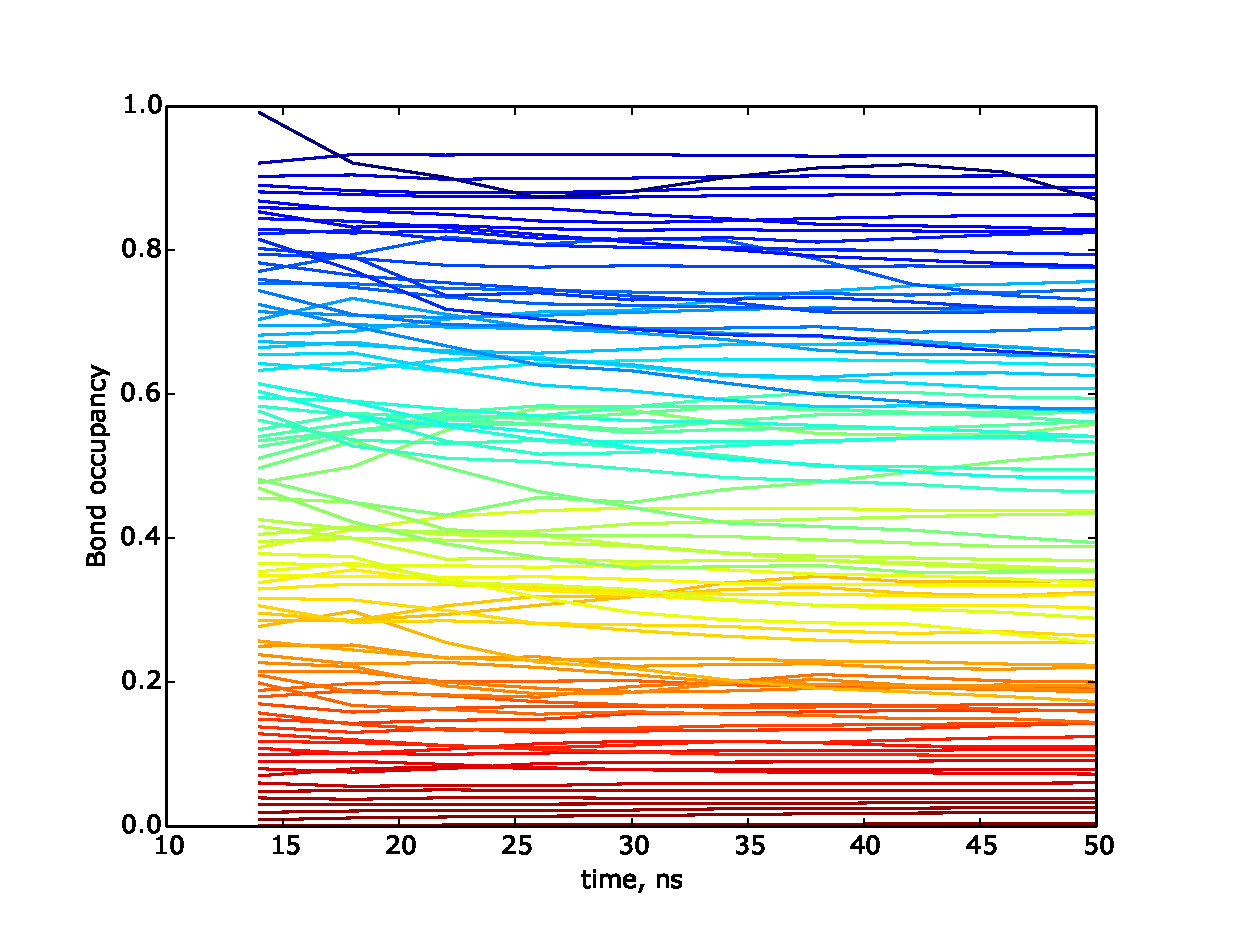
\includegraphics [width=0.75\linewidth] {md_bstab_a}
  \caption{Стабильность водородных связей между атомами белка.}
  \label{img:md_bstab_a}
\end{figure}

\begin{figure}[ht]
  \center
  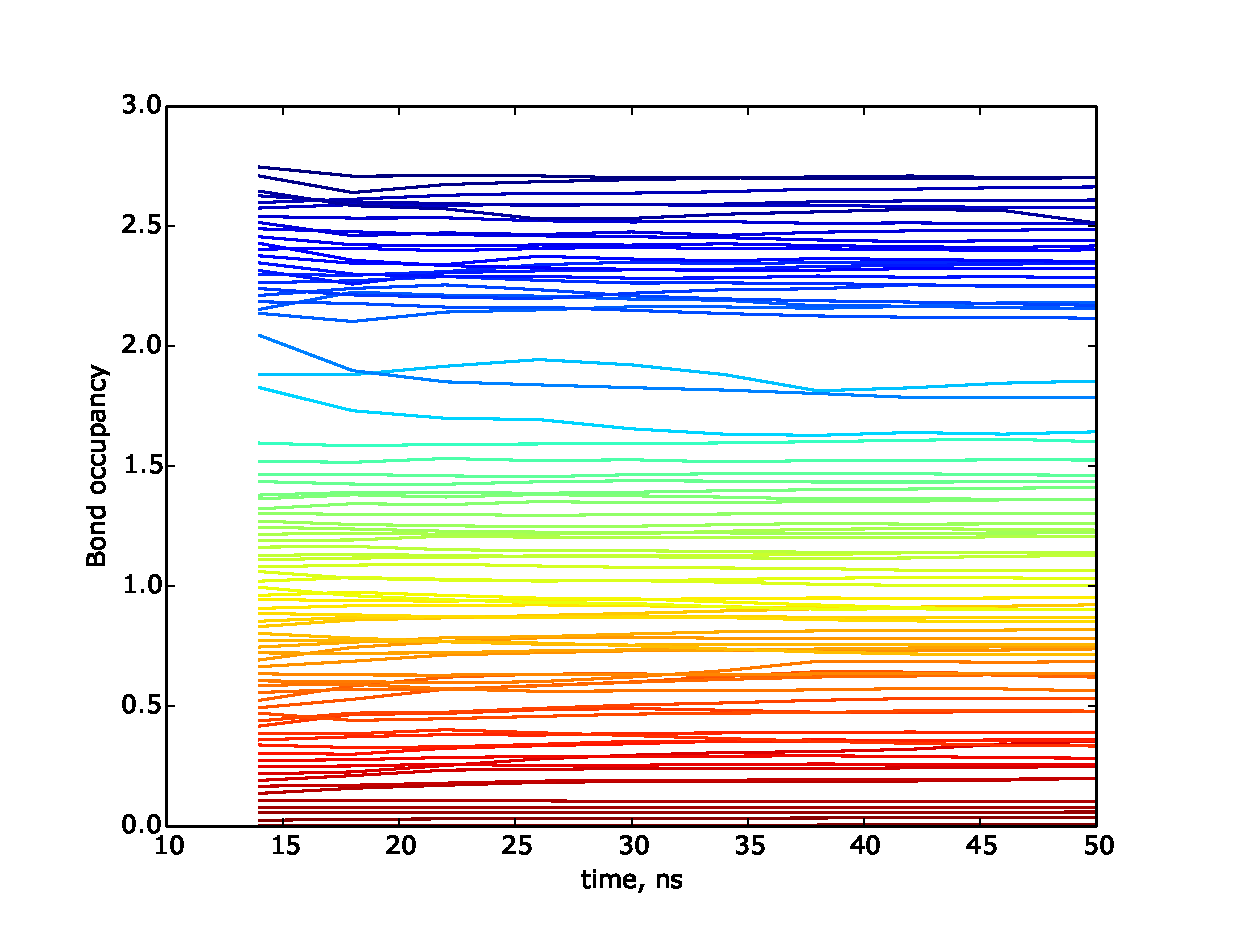
\includegraphics [width=0.75\linewidth] {md_bstab_b}
  \caption{Стабильность водородных связей между атомами белка и атомами молекул воды.}
  \label{img:md_bstab_b}
\end{figure}

\begin{figure}[ht]
  \center
  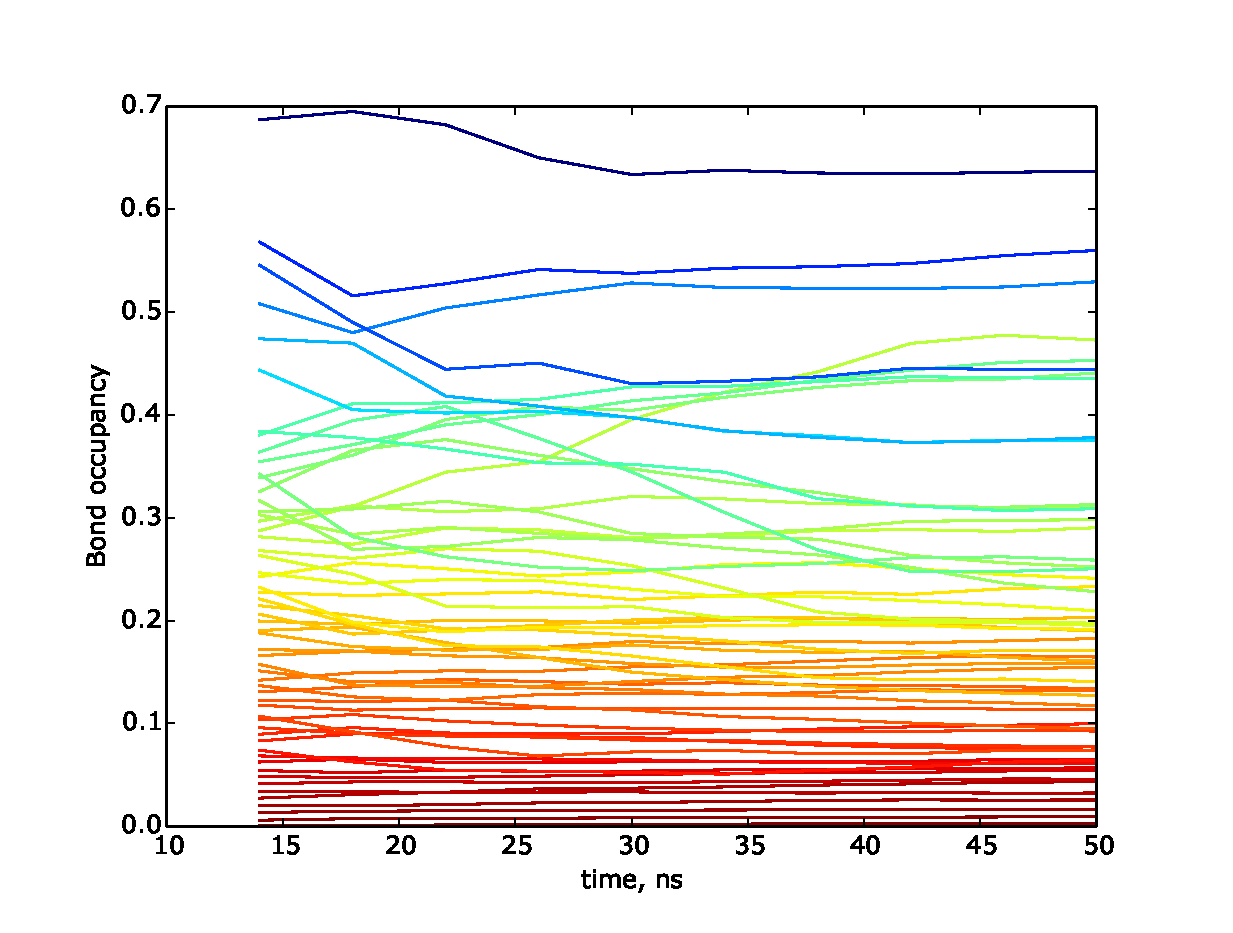
\includegraphics [width=0.75\linewidth] {md_bstab_c}
  \caption{Стабильность водных мостиков.}
  \label{img:md_bstab_c}
\end{figure}

Стабильность связей различного типа между атомами моделируемой системы в зависимости от периода моделирования отображена на Рис. \ref{img:md_bstab_a}, \ref{img:md_bstab_b}, \ref{img:md_bstab_c}. Каждая линия отражает усреднённую динамику времён существования групп связей, имеющих сходную стабильность.
        % Приложения

\end{document}
